\pdfminorversion=7
\documentclass[a4paper,10pt,titlepage,oneside,openany]{book}

\usepackage[skip=6pt]{parskip}
\usepackage[T1]{fontenc}
\usepackage[utf8]{inputenc}
\usepackage[english]{babel}
\usepackage{lmodern}
\usepackage{graphicx}
\usepackage{grffile}
\usepackage{amsmath,amssymb,amsthm,mathtools}
\usepackage{enumitem}
\usepackage{float}
\usepackage{changepage}
\usepackage[top=1in,bottom=1in,left=1in,right=1in]{geometry}
\usepackage{fancyhdr}
\usepackage[most]{tcolorbox}
\usepackage{xcolor}
\usepackage{array,booktabs,tabularx}
\usepackage{pdfpages}
\usepackage{etoolbox}
\usepackage{ragged2e}
\usepackage{comment}
\usepackage{tikz}
\usepackage[colorlinks=true,linkcolor=black,citecolor=black,urlcolor=blue]{hyperref}

\providecommand{\LILink}{https://www.linkedin.com/company/starting-finance-club-polito}
\providecommand{\IGLink}{https://www.instagram.com/sfclubpolito}
\providecommand{\Website}{https://sfclubpolito.it/}
\providecommand{\R}{\mathbb{R}}
\providecommand{\E}{\mathbb{E}}
\providecommand{\Q}{\mathbb{Q}}
\providecommand{\dd}{\,\mathrm{d}}
\providecommand{\ii}{\mathrm{i}}
\providecommand{\vega}{\mathcal{V}}
\providecommand{\Lag}{\mathcal{L}}
\providecommand{\erf}{\operatorname{erf}}
\providecommand{\citep}[1]{\cite{#1}}
\providecommand{\citet}[1]{\cite{#1}}
\DeclareMathOperator{\plim}{plim}
\DeclareMathOperator*{\argmin}{arg\,min}
\DeclareMathOperator*{\argmax}{arg\,max}
\DeclareMathOperator{\Var}{Var}
\DeclareMathOperator{\Cov}{Cov}
\DeclareMathOperator{\Corr}{Corr}
\DeclareMathOperator{\diag}{diag}
\DeclareMathOperator{\tr}{tr}

\AtBeginDocument{\justifying}
\setlength{\parindent}{0pt}
\setlength{\parskip}{6pt}
\setlength{\emergencystretch}{2em}
\graphicspath{{img/}}

\definecolor{sfblue}{HTML}{123A63}
\definecolor{sflightblue}{HTML}{EAF2F8}
\definecolor{sfgap}{HTML}{8A4B08}
\definecolor{sfgapbg}{HTML}{FFF6E5}

\pagestyle{fancy}
\fancyhf{}
\fancyhead[L]{\textbf{Starting Finance Club PoliTo}}
\fancyhead[R]{\includegraphics[height=0.65cm,keepaspectratio]{img/Logo_SFClub_Polito.png}}
\fancyfoot[C]{\thepage}
\renewcommand{\headrulewidth}{0.4pt}
\renewcommand{\footrulewidth}{0.4pt}
\setlength{\headheight}{25pt}
\setlength{\headsep}{24pt}

\fancypagestyle{plain}{%
  \fancyhf{}
  \fancyhead[L]{\textbf{Starting Finance Club PoliTo}}
  \fancyhead[R]{\includegraphics[height=0.65cm,keepaspectratio]{img/Logo_SFClub_Polito.png}}
  \fancyfoot[C]{\thepage}
  \renewcommand{\headrulewidth}{0.4pt}
  \renewcommand{\footrulewidth}{0.4pt}
}

\theoremstyle{plain}
\newtheorem{theorem}{Theorem}[chapter]
\newtheorem{proposition}{Proposition}[chapter]
\newtheorem{corollary}{Corollary}[chapter]
\theoremstyle{definition}
\newtheorem{definition}{Definition}[chapter]
\newtheorem{notation}{Notation}[chapter]
\newtheorem{example}{Example}[chapter]
\theoremstyle{remark}
\newtheorem{remark}{Remark}[chapter]

\newenvironment{pseudocode}{\par\small\ttfamily\begin{adjustwidth}{1em}{1em}}{\end{adjustwidth}\par}

\newenvironment{tightabstract}{%
  \begin{tcolorbox}[
    title={Abstract},width=0.98\textwidth,left=4mm,right=4mm,
    top=1.5mm,bottom=1.5mm,colback=white,colframe=sfblue,boxrule=0.5pt]
  \footnotesize\justifying
}{%
  \end{tcolorbox}
}

\newcommand{\chapterstatus}[1]{%
  \begin{tcolorbox}[colback=sflightblue,colframe=sfblue,boxrule=0.5pt,arc=1mm,left=3mm,right=3mm]
  \small\textbf{Working-draft status.} #1
  \end{tcolorbox}
}
\newcommand{\sourceassetnote}{%
  \begin{tcolorbox}[colback=white,colframe=black!35,boxrule=0.35pt,arc=1mm,left=3mm,right=3mm]
  \small\textbf{Asset gate.} Only figures and result tables accepted by the provenance ledger are rendered. Legacy duplicates, raw-data views and unverified outputs remain omitted; selected frozen or regenerated assets are identified in their captions.
  \end{tcolorbox}
}
\newcommand{\gapbox}[1]{%
  \begin{tcolorbox}[colback=sfgapbg,colframe=sfgap,boxrule=0.6pt,arc=1mm,left=3mm,right=3mm,title={Open evidence gap}]
  \small #1
  \end{tcolorbox}
}
\newcommand{\sourcecitation}[1]{\textsuperscript{\textcolor{black!55}{[source audit]}}}
\newcommand{\sourceref}[1]{\textit{source item}}

\makeatletter
\newenvironment{references}{%
  \chapter*{Bibliography}
  \addcontentsline{toc}{chapter}{Bibliography}
  \markboth{Bibliography}{Bibliography}
  \list{\@biblabel{\@arabic\c@enumiv}}{%
    \settowidth\labelwidth{\@biblabel{99}}
    \leftmargin\labelwidth
    \advance\leftmargin\labelsep
    \@openbib@code
    \usecounter{enumiv}
    \let\p@enumiv\@empty
    \renewcommand\theenumiv{\@arabic\c@enumiv}}
  \sloppy
  \clubpenalty4000
  \@clubpenalty\clubpenalty
  \widowpenalty4000
  \sfcode`\.\@m
}{%
  \def\@noitemerr{\@latex@warning{Empty `references' environment}}
  \endlist
}

% Preserve the accepted Research-template vertical fingerprint.
\patchcmd{\@makechapterhead}{\vspace*{50\p@}}{\vspace*{-18\p@}}{}{}
\patchcmd{\@makeschapterhead}{\vspace*{50\p@}}{\vspace*{-18\p@}}{}{}
\patchcmd{\@makechapterhead}{\huge}{\fontsize{17}{20}\selectfont\bfseries}{}{}
\patchcmd{\@makechapterhead}{\Huge}{\fontsize{20}{24}\selectfont\bfseries}{}{}
\patchcmd{\@makeschapterhead}{\Huge}{\fontsize{20}{24}\selectfont\bfseries}{}{}
\patchcmd{\@makechapterhead}{\vskip 20\p@}{\vskip 6\p@}{}{}
\patchcmd{\@makechapterhead}{\vskip 40\p@}{\vskip 10\p@}{}{}
\patchcmd{\@makeschapterhead}{\vskip 40\p@}{\vskip 10\p@}{}{}
\makeatother

\title{Stochastic Framework for\\Barrick Mining Corporation Valuation}
\author{%
\scriptsize
\begin{tabular}{ll}
\textbf{Team 1} & Stefano Falcione; Marco Fracca\\
\textbf{Team 2} & Filippo Triassi; Giorgio Zoccatelli\\
\textbf{Team 3} & Andrea Rostagno; Francesco Florio\\
\textbf{Team 4} & Giacomo Scali; Jacopo Foralosso\\
\textbf{Team 5} & Federico Vesco; Lorenzo Pietra; Bader Moussaif\\
\textbf{Team 6} & Davide Sisto; Matteo Armando\\
\textbf{Team 7} & Davide D'Amico; Pietro Weisz\\
\textbf{Team 8} & Salvatore Gabriele Messina; Alessandro Coco
\end{tabular}
}
\date{TBD --- \textbf{Draft: Not ready for publication}}

\newcommand{\abstracttext}{%
This study constructs and audits a stochastic valuation architecture for
Barrick Mining Corporation within Starting Finance Club PoliTo Research. Eight
teams contribute probability, econometrics, Monte Carlo, historical gold
dynamics, stochastic volatility and jumps, option calibration, purpose-built
mine forecasts and discounted cash flow. Unification assigns each variable to
one source authority and links the layers through explicit date, unit, measure
and accounting contracts. Its central design choice is separation: Black--Scholes/
GBM, Heston, Bates--Poisson and Full Bates--Hawkes are four Team 8 engines for
the \emph{gold-price layer} in the frozen baseline. A separate extension fits
the same model families to copper options and adds three attributable copper
mines. The price models do not model production or costs.
Barrick's Q1--Q2 2026 actual production and Cost of Sales form the
current stub; Team~4 forecasts begin at Q3 and remain explicitly labelled.
The unified tax, growth, ROIC, stochastic WACC, terminal-value and
equity-bridge adaptation is common. Team~4's legacy NSS, IV, GBM and
illustrative stochastic EBITDA artifacts are excluded. In their place, the
current Team~8 build fits an independent Nelson--Siegel--Svensson curve to
14 U.S. Treasury tenors dated 2 September 2026. Its 2.0608 basis-point RMSE
is measured against a continuously compounded par-yield proxy, not a
bootstrapped zero curve. The same curve supplies option-maturity rates and
integral-preserving quarterly forward rates. The dense GLD surface contains
605 eligible calls across 12 expiries and 146 strikes; a fixed Chebyshev sample
selects 64 actual contracts across eight expiries and 20 strikes.
Heston has the lowest current in-sample IV RMSE, 49.4881 basis points, against
97.2107 for Black--Scholes, 54.6273 for Bates--Poisson and 52.9714 for
Full Bates--Hawkes. The latter is the primary structural scenario because it
has the lowest date-equal rolling OOS IV RMSE, 65.0507 basis points across
30 forecast origins and 4,667 common forecasts. No model beats interpolated
IV-surface persistence. Its current branching ratio is 0.5569, below unity;
this snapshot does not establish parameter stability across regimes.
The accepted comparison uses 8,192 paths over 20 quarters and one common WACC
shock array. The frozen market reference is the USD~44.13 close on 2 September
2026. Under Full Bates--Hawkes, conditional P10/P25/P50/P75/P90 values are
USD~3.13/14.85/35.14/65.24/104.72. The close is USD~8.99, or 25.58\%, above
the median, lies at the 59.24th percentile and is exceeded by 40.76\% of paths.
The four medians range from USD~35.14 to USD~35.87. This comparison does not
establish market mispricing. Only GLD/$\mathbb Q$ distributional shape is
transferred to paths restarted at Barrick's Q2 average realised-price anchor
of USD~4,417/oz; no one-for-one GLD conversion or validated
$\mathbb Q$-to-$\mathbb P$ mapping is performed. The surface, Treasury curve
and equity close share 2 September, while the anchor quarter ends 30 June.
Persistent costs grant no additional technology-driven reductions, making
the assumption prudential relative to otherwise identical efficiency scenarios,
not a mathematical lower bound on value.
Component margin and FCFF remain proxies; debt, cash, minorities,
non-operating assets and other equity adjustments are zero placeholders, and
the 1,675.51 million-share input is unreconciled. The 86-bar Barrick window and
August market-context diagnostics are historical, not current calibration evidence. Timestamped
news and an NLP/ML
filtration for geopolitical and macroeconomic shocks remain absent.
Accordingly, the reported distributions are controlled research sensitivities,
not physical forecasts, confidence intervals, fair values, targets or
investment advice.}

\makeatletter
\renewcommand{\maketitle}{%
\begin{titlepage}
  \thispagestyle{empty}
  \centering
  \vspace*{-0.7cm}
  \includegraphics[width=2.55cm]{img/Logo_SFClub_Polito.png}\\[0.25cm]
  {\fontsize{23}{26}\selectfont\bfseries \@title\par}
  \vspace{0.22cm}
  {\normalsize\textbf{Contributing authors}\par}
  \vspace{0.10cm}
  {\@author\par}
  \vspace{0.12cm}
  {\small\@date\par}
  \vspace{0.14cm}
  {\large\textbf{Starting Finance Club PoliTo}\par}
  \scriptsize
  LinkedIn: \url{\LILink}\quad
  GitHub: \url{https://github.com/StartingFinanceClubPoliTo/Research}\\[-1pt]
  Instagram: \url{\IGLink}\quad Website: \url{\Website}
  \vspace{0.18cm}
  \begin{tightabstract}
  \abstracttext
  \end{tightabstract}
\end{titlepage}
}
\makeatother

\hypersetup{
  pdftitle={Stochastic Framework for Barrick Mining Corporation Valuation},
  pdfsubject={LSE-refreshed conditional multi-model valuation with explicit evidence gaps},
  pdfauthor={Starting Finance Club PoliTo --- Research Area}
}

\begin{document}

\hypersetup{pageanchor=false}
\includepdf[pages=1,fitpaper=true,pagecommand={\thispagestyle{empty}\begin{picture}(0,0)\put(225,-240){\makebox(0,0){\colorbox{white}{\textbf{Draft: Not ready for publication --- TBD}}}}\end{picture}}]{Copertina_research.pdf}
\clearpage
\maketitle

\frontmatter
\hypersetup{pageanchor=true}
\pagenumbering{roman}
\setcounter{page}{1}

\input{chapters/00-discoveries-at-a-glance}

\tableofcontents
\thispagestyle{plain}

\mainmatter
\setcounter{page}{1}

\part{Origins of the Research, Gold and Barrick}
\chapter{From SF Research to the Integrated Barrick Project}
\chapterstatus{The project history in this chapter follows the mandate supplied
by SF Research. The methodological map is a source-grounded synthesis of Teams
1--8 and the accepted current evidence; it does not promote the conditional
corporate proxy to a filing-reconciled valuation.}

\section{Research question, community and valuation object}

% Sources: CONTENT-LEDGER BG-U-01, BG-U-10--14; CL-001/002/011/013;
% Team 8 T8-17--19; Team 4 MAP-T4-08--12; Team 5 T5-02--19;
% SF Research complete guide, project organisation and unification workflow.
SF Research did not begin as a preassembled quantitative-finance laboratory.
It originated as a comparatively vertical group, strongly represented by
management-engineering students and initially centred on events and financial
education. Research activity first appeared through short studies developed by
small groups over roughly monthly horizons. As contributors with different
academic paths entered the area, those isolated exercises gradually revealed a
larger opportunity: to build a common annual project in which every member
could contribute while learning how separate disciplines meet in a real
valuation problem.

That evolution matters because the project's main advantage is
interdisciplinarity. A mathematics curriculum can reasonably treat probability,
analysis or numerical foundations as prerequisites; a management curriculum
can do the same with accounting and valuation; a computing curriculum can
assume familiarity with implementation. The team deliberately avoided those
silent assumptions. The project was designed from the bottom up so that it
could extend, rather than merely repeat, the contributors' university
programmes and introduce models and techniques that many of them had not met
in formal courses.

The resulting chain joins economics and corporate finance with mathematics,
econometrics, statistics and probability, stochastic methods, numerical
methods, optimisation, operations research and computing. At university these
subjects are often taught as distinct modules. In the Barrick project they are
forced to interact: probability supplies the language of uncertainty;
econometrics tests the historical series; stochastic calculus defines the
continuous-time models; numerical methods make calibration and simulation
possible; optimisation estimates parameters; operational modelling converts
gold, production and costs into margins; and corporate finance closes the DCF.
The thesis is therefore both a valuation study and a record of how theoretical
ideas become mutually dependent when applied to one object.

The integrated research question is: \emph{how can uncertainty in commodity
prices, production, costs and corporate assumptions be propagated into a
distribution of Barrick free cash flow and value without confusing
risk-neutral option information with a physical operating forecast?} The
object is not a point price produced by an isolated option model. It is a
conditional distribution of enterprise value and, after a separately verified
capital bridge, equity value and value per diluted share. The comparison with
the observed market price is therefore a dated diagnostic inside a declared
assumption set, not a target price or a recommendation.

This project was developed within Research, the Starting Finance Club PoliTo
area dedicated to collaborative quantitative, economic, financial and
methodological projects. Its members bring heterogeneous backgrounds---from
management engineering and mathematics to data science, computational methods
and quantitative finance---so the research process is organised around
knowledge sharing rather than an assumed common starting point. The practical
objective is to establish enough shared language and method for contributors
with different training to make a verifiable contribution, while keeping
technical depth accessible to readers who did not participate in the project.
This description concerns how the work was organised; it is not presented as a
formal institutional mission or organisational chart.

That collaborative setting is material to the valuation design. The commodity
block must state whether paths are risk-neutral, physical or explicit
scenarios; the operating block must state production, cost and realised-price
units; the accounting block must reconcile operating margin, depreciation,
taxes and reinvestment; and the valuation block must state discounting,
terminal closure and every enterprise-to-equity adjustment. A result becomes
economically interpretable only when contributors working on different modules
use the same date, perimeter, currency, notation and manifest. The research
question is therefore also an integration question: whether heterogeneous
analytical work can be connected without hiding disagreements in definitions
or silently filling missing data.

\section{From eight autonomous studies to one chain of evidence}

% Sources: CONTENT-LEDGER authority table; MAP-T1--T4; T5-01--T8-20;
% SF Research complete guide, unification and review workflow.
The eight source studies divide the problem into complementary modules. Team 1
provides probability, measure and Black--Scholes foundations; Team 2 provides
regression and linear time-series methods; Team 3 provides Monte Carlo and
simulation diagnostics; Team 4 maps production, cost and price scenarios into
an operating layer; Team 5 supplies DCF, FCFF, WACC and stochastic-valuation
concepts; Team 6 develops stochastic variance, jumps and Fourier pricing; Team
7 supplies historical gold, dependence and volatility evidence; and Team 8
compares option-surface models and produces risk-neutral GLD paths. These were
autonomous studies with different immediate questions, conventions and
validation states, not chapters originally written as a single sequential
paper.

Unification was consequently treated as a separate research phase rather than
as copy-and-paste assembly. Before drafting the integrated argument, the work
froze the admissible sources and material claims, assigned an authority to each
concept, and classified outputs as theoretical, synthetic, legacy empirical,
current empirical or newly generated. Data and notation contracts then made
dates, currencies, units, measures and interfaces explicit. Source-model
implementations were preserved and subjected to parity tests before being
connected to the unified runner, while the current LSE refresh was recorded as
a separate evidence layer so that a new market observation could not be
mistaken for a re-estimation of every legacy study.

The execution itself followed two connected workstreams. The code stream built
and tested the valuation pipeline, generated tables and figures from accepted
manifests, and exposed unresolved inputs instead of replacing them with silent
assumptions. The writing and LaTeX stream harmonised notation, removed
duplication, created transitions and kept claims tied to their evidence status.
Technical review checked models, calculations and reproducibility; editorial
review checked scope, language and reader navigation; final quality assurance
tested both the compiled artifact and the consistency between prose, tables,
figures and generated outputs. Section~\ref{sec:team-study-synthesis} makes the
resulting roles and validation states directly comparable.

\section{Contribution, falsifiable boundaries and roadmap}

% Sources: VAL-001 gate sequence in GAP-REGISTER; CL-001/005/012/013.
The first contribution is an auditable handoff from option-implied dynamics to
corporate quantities. The second is an evidence hierarchy that separates
source-model parity, market-data validity, statistical fit, predictive tests,
numerical convergence and accounting reconciliation. The third is a reporting
contract: a stochastic valuation must expose its median and tails, the
contemporaneous market-price reference and the assumptions that move the
distribution, rather than presenting a single estimate with false precision.
Together, these contributions make disagreement inspectable: a reader can see
whether a result changes because of market evidence, model form, operating
assumptions, accounting treatment or the equity bridge.

The same structure creates falsifiable boundaries. Better option fit does not
prove better out-of-sample forecasts; better forecasts do not prove a valid
GLD-to-realised-gold bridge; a valid commodity bridge does not prove the mine
or accounting perimeter; and a coherent enterprise value does not determine
equity value until net debt, minorities, non-operating assets and diluted
shares are reconciled. Each boundary has a corresponding validation gate in
Chapter 12. Failure at a later gate does not erase an earlier technical
result, but it narrows the conclusion that the integrated study may draw from
that result.

The thesis follows the same chain. Part I reconstructs the genesis of the
research, the monetary and macroeconomic role of gold, and the Barrick
valuation perimeter. Part II consolidates the mathematical, econometric and
numerical prerequisites from the bottom up. Part III first tests the legacy
gold series with discrete-time methods, then introduces the affine
stochastic-volatility and jump model ladder, and finally calibrates and
compares the models on the option surface. Part IV carries the admitted gold,
production and cost paths through component margin and DCF, validates the integrated
experiment and closes with limitations and future research. No part of the
study provides a buy, sell or hold recommendation.

\input{chapters/02-gold-regimes-debasement}
\chapter{Barrick Mining Corporation and Valuation Perimeter}
\chapterstatus{Legal identity and listing continuity are verified from Barrick's
official releases. The gold operating perimeter, variable definitions, units,
data window and forecast frequency follow the Team~4 source study
\cite{team4}; ownership shares, accounting treatment and 2025 structural events
are documented in Barrick's 2025 Annual Report \cite{barrick-ar-2025}.
A separate copper extension is identified explicitly. The financial perimeter
and equity bridge remain controlled inputs requiring reconciliation.}

\section{Corporate identity and the choice of case study}
\label{sec:company-identity}

The project retained its historical working name, ``Barrick Gold'', but the
legal issuer is now \emph{Barrick Mining Corporation}. Shareholders approved
the change from Barrick Gold Corporation on 6 May 2025. Trading under the new
name began on 9 May 2025; the New York Stock Exchange ticker changed from
\texttt{GOLD} to \texttt{B}, while the Toronto Stock Exchange ticker remained
\texttt{ABX} \cite{barrick-name-2025}. The distinction matters whenever a
market-price series is stitched across the corporate action.

The corporate action does not interrupt the operating series. Team~4 extracted
its mine-level data from the quarterly reports published on the company's
investor website, under the Barrick Gold Corporation name until 2025 and under
the Barrick Mining Corporation name thereafter; both refer to the same issuer.
Team~4 adopts the process and cost definitions of the 2024 Annual Report and
checks its first forecast year against the 2025 report's guidance
\cite{team4,barrick-ar-2025}. The name and ticker change affects the market
series of Section~\ref{sec:lse-current-diagnostics} and the equity bridge,
but not the operating panel's continuity.

Barrick is a gold and copper exploration, development and mining company
\cite{barrick-about-2026}. Its original Team~4 operating layer is narrower:
eight gold mines, excluding copper and the remaining gold assets \cite{team4}.
Section~\ref{sec:copper-extension} adds Lumwana, Zald\'ivar and Jabal Sayid as
an explicit copper scenario, without rewriting the frozen gold experiment.
Neither perimeter represents every corporate asset or a reconciled claim on
the whole company. The case connects commodity prices, production and costs
to component margin and a conditional DCF, bringing the team's valuation
interests into its stochastic modelling framework.

\section{The company perimeter is a model input}
\label{sec:company-perimeter}

% Sources: Team 4 Sections 1.1.2--1.1.3, 2 and 3.1; Annual Report 2025,
% MD&A mine tables and Note 2; 2026Q1--Q2 mine statistics in Chapter 10.
A valuation must freeze, by asset and date, the ownership and reporting basis,
status and currency. These determine which volumes, costs, taxes, royalties,
cash flows, debt claims and shares enter its numerator and denominator.
Table~\ref{tab:company-operating-perimeter} records the gold perimeter.

\paragraph{Admitted assets.}
Bulyanhulu, Carlin, Cortez, Kibali, Loulo--Gounkoto, North Mara, Pueblo Viejo
and Turquoise Ridge form the base of the gold operating computations,
including Chapter~10's production-weighted cost master chain. The source
excluded copper and smaller gold operations \cite{team4}; this modelling
choice does not demonstrate that copper is economically negligible.
The eight mines produced 622 and 711 thousand attributable ounces in 2026Q1
and 2026Q2 against company gold totals 719 and 796 thousand ounces
(Chapter~10): 86.5\% and 89.3\% of attributable gold production. These are
gold-volume coverage ratios, not corporate-revenue or value coverage.

The frozen executable gold vector uses company totals of 719 and 796 koz,
and company-wide CoS of USD~1,922 and 1,993/oz, for its first two quarters.
From 2026Q3 it uses the eight-mine Team~4 forecast. Its first two actual
quarters therefore have a broader asset scope than its forecast perimeter.
This scope break remains explicit in the paired copper experiment; the
eight-mine coverage table does not reconcile it. A consistent mine-level
actual vector and matching aggregate costs are required before the baseline
can be read as a strict eight-mine valuation.

\begin{table}[H]
\centering
\caption{Team~4 gold perimeter: Barrick's interest and accounting treatment
at 31 December 2025 \cite{team4,barrick-ar-2025}.}
\label{tab:company-operating-perimeter}
\small
\renewcommand{\arraystretch}{1.12}
\begin{tabularx}{\textwidth}{@{}>{\raggedright\arraybackslash}p{2.15cm}%
>{\raggedright\arraybackslash}p{1.75cm}%
>{\raggedright\arraybackslash}p{3.85cm}%
>{\raggedright\arraybackslash}X@{}}
\toprule
\textbf{Mine} & \textbf{Location} & \textbf{Barrick interest and accounting}
& \textbf{Source-specific notes} \\
\midrule
Carlin & Nevada, USA & 61.5\% through Nevada Gold Mines; consolidated with
38.5\% non-controlling interest (Newmont). & Reference mine: 28 quarters,
2019Q1--2025Q4; simulated recovery in $[0.71,0.85]$. \\
Cortez & Nevada, USA & 61.5\% through Nevada Gold Mines; as Carlin. &
Winter seasonality in throughput. \\
Turquoise Ridge & Nevada, USA & 61.5\% through Nevada Gold Mines; as Carlin. &
Winter seasonality in throughput. \\
Pueblo Viejo & Dominican Republic & 60\%; consolidated with 40\%
non-controlling interest (Newmont). & Wet-season throughput seasonality. \\
Kibali & DR Congo & 45\%; equity-accounted joint venture (AngloGold Ashanti
45\%, DRC Government 10\%). & Outside consolidated revenue and CoS;
proportionate in attributable per-ounce metrics. \\
Loulo--Gounkoto & Mali & 80\%; consolidated with 20\% non-controlling
interest; deconsolidated 16 June, reconsolidated 16 December 2025. & Suspended
from 14 January; 29 thousand ounces in 2025; wet-season seasonality. \\
North Mara & Tanzania & 84\%; consolidated with 16\% non-controlling
interest (Government of Tanzania). & 25 quarters from separate reporting
in 2019Q4. \\
Bulyanhulu & Tanzania & 84\%; as North Mara. & -- \\
\bottomrule
\end{tabularx}
\end{table}

\paragraph{Reporting basis.}
The operating layer is attributable. Mine-level MD\&A tables report ore
processed, grade, recovery, ounces produced and sold and CoS on Barrick's
share: 61.5\% for the Nevada mines, 60\% Pueblo Viejo, 45\% Kibali and
84\% for the Tanzanian mines \cite{barrick-ar-2025}. Per-ounce CoS uses
attributable ounces sold. Ore and the ounces it generates share one basis;
Section~\ref{sec:company-operating-quantities}'s production identity is
dimensionally consistent. Grade and recovery are ratios. Ownership must not
be applied again to already attributable volumes.

Legal ownership does not always equal the economic share. Under the Tanzanian
agreement the government receives half of economic benefits through taxes,
royalties, clearing fees and cash distributions after capital recoupment;
earnings are recorded on Barrick's 84\% equity interest
\cite{barrick-ar-2025}. Volume reporting is suitable for production and cost;
the cash-flow split belongs to the tax and bridge layers.

\paragraph{Data window.}
The quarterly estimation window starts in 2019 and ends in 2025Q4 even where
longer histories exist \cite{team4}. Leading missing production-driver values
are removed mine by mine: Carlin contributes 28 quarters, North Mara 25 from
2019Q4. A common starting year therefore does not imply identical effective
samples for every driver. The 2026Q1--Q2 mine statistics replace the first
two forecast quarters as actuals; forecasts from 2026Q3 remain as originally
estimated (Chapter~10).

\section{Operating quantities supplied by the source programme}
\label{sec:company-operating-quantities}

% Sources: Team 4 Sections 1.1.3, 2.2--2.4, 3.1--3.2 and 4.1;
% Annual Report 2025, Production Costs and mine tables.
Production and CoS are forecast separately, mine by mine, on 20 quarters
from 2026Q1 to 2030Q4. Annual quantities sum four quarters. The price comes
from Team~8 in Chapter~9; Team~4's standalone demonstrator is excluded.

\paragraph{Production.}
Quarterly production of mine $i$ is built from three physical drivers,
\begin{equation}
\mathrm{Prod}_{i,t}=\frac{\kappa}{c}O_{i,t}G_{i,t}R_{i,t},
\qquad\kappa=0.91,\quad c=31.1035~\text{g/oz},
\label{eq:company-production-identity}
\end{equation}
where $O$ is ore processed in tonnes, $G$ processed grade in grams per tonne
and $R\in(0,1)$ recovery. Their product is recovered gold in grams; $c$
converts grams to troy ounces. The realisation factor $\kappa$ is the mean
mine ratio of realised to theoretical production, absorbing lags such as
stockpiling, heap leaching and autoclave residence \cite{team4}. The source
uses rounded $31.11$, lowering output approximately $0.02\%$; conversion
is from grams, not tonnes as stated in its text. Ore uses
SARIMA$(1,0,1)(1,0,0)_4$, grade AR(1) without seasonal terms, and recovery
uniform historical bounds widened by $\pm1\%$, truncated to $[0.50,1.00]$.
Production bands are 80\% Goodman product-variance intervals under
independence (Chapter~10).

\paragraph{Costs.}
CoS is USD per attributable ounce sold, excluding closure or care-and-
maintenance sites. The 2024 definition used by Team~4 includes site costs,
royalties, depreciation and community relations \cite{team4}; the 2025 report
also identifies mining and production taxes. Consolidated gold CoS in 2025
was USD~7,357 million: site costs 5,056; depreciation 1,588 (21.6\%);
royalties 540 (7.3\%); mining and production taxes 132; community relations
41 \cite{barrick-ar-2025}. The production-weighted log master chain is
ARIMA$(3,1,0)$ with drift, projected to each mine by
$\beta_i=0.67\,\sigma(r_{i,t})/\sigma(r_{\mathrm{global},t})+0.33$ and anchored
at 2025Q4. Cost bands are 95\%, versus production's 80\%.

\paragraph{Operating output.}
For quarterly gold price $P_t$ in USD/oz, the source passes
\begin{equation}
\mathrm{CM}_t=(P_t-\mathrm{CoS}_t)\mathrm{Prod}_t
\label{eq:company-component-margin}
\end{equation}
to valuation. Because CoS contains depreciation, this is after-depreciation
\emph{component margin}, not EBITDA despite the source label \cite{team4}.
Nevada Gold Mines' 2025 mine income USD~3,141 million plus depreciation 568
gives reported EBITDA 3,709 \cite{barrick-ar-2025}. The corporate gold cost
mix puts depreciation near one fifth of CoS. Nor is the margin reconciled
EBIT: G\&A, exploration, project expenditure and other items are absent.
CoS is per ounce \emph{sold}, while the identity multiplies ounces
\emph{produced}. Forecast royalties are fixed per ounce, although Barrick
attributes about USD~55/oz of the 2025 CoS increase to higher royalties from
higher realised gold prices \cite{barrick-ar-2025}. Chapter~11 must reconcile
these mismatches before the proxy becomes accounting cash flow.

\begin{table}[H]
\centering
\caption{Operating contract of the original Team~4 gold module.}
\label{tab:company-operating-contract}
\small
\renewcommand{\arraystretch}{1.12}
\begin{tabularx}{\textwidth}{@{}p{2.15cm}X X@{}}
\toprule
\textbf{Dimension} & \textbf{Team~4 specification} &
\textbf{Reconciliation still required} \\
\midrule
Perimeter & Eight gold mines, attributable; copper and other gold assets
absent from source module. & Separate copper extension; other assets,
per-share basis and North America IPO. \\
Frequency and horizon & Quarterly estimation 2019--2025; 20 quarters to
2030Q4; annual sums; Q1--Q2 2026 actuals. & No mine-life model supports a
terminal assumption beyond 2030. \\
Production & $O$ in t, $G$ in g/t, $R$ decimal, output oz; seasonal ore,
AR(1) grade, uniform recovery; 80\% Goodman bands. & Produced versus sold;
only point forecasts enter frozen valuation. \\
Costs & USD/oz CoS includes depreciation and royalties; log ARIMA$(3,1,0)$
with drift, $\beta$ scaling, Q4 2025 anchors; 95\% bands. & D\&A, royalties,
taxes, capex, G\&A, exploration and exceptional anchors; no AISC model. \\
Commodity price & Source only: GBM at USD~4,677/oz on 2 April 2026 using GLD
per-expiry volatility; excluded here. & Team~8 shapes at Q2 realised gold
USD~4,417/oz; no GLD-level conversion; realised basis, hedging and measures. \\
Operating output & After-depreciation component margin, called EBITDA in
source. & EBIT, taxes, working capital and capex bridge. \\
Dependence & Ore--grade $r\approx-0.45$, ore--recovery $r\approx-0.17$;
cost PC1 41.22\%, Bartlett $p=0.0186$; fixed operating vectors in valuation.
& Joint simulation, production response and royalty--price link. \\
\bottomrule
\end{tabularx}
\end{table}

\section{Financial and structural perimeter}
\label{sec:company-financial-perimeter}

The financial perimeter fixes statements, currency and scale for taxes,
reinvestment and capital costs, and debt, leases or equivalent claims,
non-controlling interests, non-operating assets and diluted shares. Model and
market claims must refer to the same security and date.

Barrick consolidates the Nevada, Pueblo Viejo, Loulo--Gounkoto and Tanzanian
operations and equity-accounts Kibali \cite{barrick-ar-2025}. Here flows
already represent Barrick's share. Deducting those same partners' interests
again would double count their exclusion. Consolidated cash and debt include
full subsidiary balances and exclude Kibali's; claims must be restated
consistently with attributable flows, including corporate-level claims,
not multiplied mechanically by one aggregate ownership fraction.

The 1,675.51 million diluted-share proxy remains unreconciled (Chapter~11).
Shares claim the whole company, whereas the gold baseline and gold-plus-
copper extension cover defined subsets. Per-share division allocates a
perimeter proxy; it does not yield full-company equity fair value. The copper
extension reports aggregate operating-value proxies without per-share targets.

Loulo--Gounkoto was suspended 14 January 2025, placed under provisional
administration and deconsolidated 16 June, then returned to Barrick control
16 December following the agreement announced 24 November. On 1 December
2025 the Board authorised preparation of an IPO of an entity holding its
Nevada Gold Mines and Pueblo Viejo interests plus Fourmile, expected by late
2026 with Barrick retaining control \cite{barrick-ar-2025}. External ownership
would change effective look-through interests in four modelled mines. The
December 2025 percentages cannot simply be carried beyond completion.
The 2025 Hemlo and Tongon sales lie outside the eight-mine vector.
The annual report alone does not fix IPO status on 2 September 2026.
The 28 April update and the 10 August Q2 release still describe a planned
minority-stake IPO expected by year end \cite{barrick-ipo-2026,barrick-q2-release-2026}.
The latter also announces Newmont's consent, an early contribution of excluded
properties to Nevada Gold Mines and a USD~1.95 billion top-up payment. Those
events require their own asset, timing and cash-bridge reconciliation; they
do not authorise a silent change to the frozen eight-mine forecast vector.
The 2026Q2 operating release predates the 2 September market snapshot, but its
reporting-period end, publication date and October retrieval remain distinct.

\gapbox{Freeze date, currency and scale; restate debt, cash, other claims and
non-operating assets consistently with attributable flows, without deducting
the same partners' interests twice; reconcile diluted shares; verify North
America IPO status at the valuation date and resulting look-through ownership;
document the security and corporate-action policy of the market comparison.}

\section{Risk boundary and permitted use}
\label{sec:company-risk-boundary}

The gold mines span Nevada, the Dominican Republic, Mali, Tanzania and the
DRC. Team~4's lag-four throughput term captures winter or wet-season
constraints. Structural events are not endogenous: the source treats the
Loulo--Gounkoto suspension as a mine-specific shock absorbed geographically
and over time, and simultaneous failures as negligible \cite{team4}.
This is an assumption, not an estimated geopolitical-risk bound.

Production diversification does not imply independent costs. Bartlett's test
rejects independence ($p=0.0186$); PC1 explains 41.22\% of quarterly cost
shocks, the first two components 62.79\% \cite{team4}. Shared cost shocks
motivate the master chain and remain systematic across the perimeter.

Cost paths start at 2025Q4. Loulo--Gounkoto's USD~4,151/oz CoS includes the
inventory fair-value increment on reconsolidation, versus cash costs
USD~1,448/oz. Its 2026 CoS guidance USD~2,860--3,140/oz still includes higher
purchase-price-allocation depreciation \cite{barrick-ar-2025}. Projecting
that anchor carries an exceptional effect forward; it needs a separate
normalisation check. This edit does not silently alter the frozen vector.

Reserve life is outside the model. Grade is stationary over five years under
feed-blending arguments; depletion, closure, high-grading, throttling and
care and maintenance are not endogenous \cite{team4}. Neither that model
nor flat extension of observed copper forwards supplies mine-life evidence
for perpetuity. The copper comparison uses a finite five-year primary
horizon and separate terminal sensitivities. Until accounting, structural
and measure bridges are admitted, the document defines a research contract
and its failure conditions, not a final target value.

\section{Data, Provenance and Experimental Design}
\label{sec:data-design}
\chapterstatus{Editorial synthesis of the accepted provenance, notation and gate contracts. Provider-specific values remain governed by their source freezes.}

\subsection{Data universe and dates}

The legacy corpus contains different evidence domains: long-run gold and silver
time series, London Stock Exchange market and option inputs, mine-level
operating data and synthetic DCF examples. Each retains its own provider,
frequency, date range, unit and measure. The operating domain is quarterly and
mine-level: Team~4 estimates on 2019Q1--2025Q4 Barrick reports, with shorter
effective samples where leading observations are missing; 2026Q1--Q2 enter
as actuals and forecasts cover 2026Q3--2030Q4
(Section~\ref{sec:company-perimeter}). The 2 April 2026 GLD option snapshot
and standalone Team~4 GBM paths are a separate legacy domain, excluded from
the integrated valuation \cite{team4}. Gold histories, option-calibration
surfaces and operating panels are not pooled.

The copper extension is another declared experiment: historical HG/HXE
bid/ask surfaces, contemporaneous matching futures and date-specific Treasury
curves are distinct from both GLD and the mine panel. Its preliminary temporal
pilot samples ten dates across 9 July--2 September 2026, including the final
three consecutive dates, with approximately 100 spaced real locations per
date. It is not a reproduction of the 31-date gold OOS panel. Missing, stale
or wide-spread quotes remain exclusions; no synthetic quotes complete a date.
The surviving contract catalogue prevents a complete point-in-time universe
and expired-option history is unavailable from this API
\cite{ib-historical-limitations}. Admitted dates and actual forecast gaps are
reported in Section~\ref{sec:copper-extension}.

\subsection{Provenance and reproducibility}

Every quantitative result admitted to the final study must be traceable through an input hash, as-of date, configuration, seed where applicable, executable stage, output path and tolerance. Exact reuse identifies material preserved from a source article; edited reuse identifies rearrangement or notation harmonisation; recomputed identifies a result created by a frozen executable run. A gap never authorises a fabricated value.

\subsection{Common notation, units and model interfaces}

The notation distinguishes the physical measure $\mathbb P$ from the pricing
measure $\mathbb Q$, GLD in USD/share from gold in USD/oz, annualised decimals
from percentage points, and enterprise from equity value. Production is
$\mathrm{Prod}$ or italic $Q$ in Chapter~11, distinct from $\mathbb Q$.
Ore is in tonnes, grade in g/t, recovery decimal, and production in troy
ounces of $31.1035$ grams, usually reported in thousands. Gold CoS is USD
per attributable ounce sold. Copper prices and CoS are USD/lb, attributable
sales are kt, and $1~\mathrm{t}=2204.6226218488~\mathrm{lb}$. Values use an
explicit scale, normally USD millions; per-share values require a reconciled
diluted-share denominator. Already attributable volumes are never scaled by
ownership twice.

\subsection{Evaluation design}

Model fit, predictive performance, numerical convergence and economic sensitivity are separate questions. In-sample residual improvement is not evidence of out-of-sample superiority. Likewise, source-model parity is a prerequisite for integration, not a new economic finding.

Error metrics must use the scale relevant to the valuation. Team~4's
12-quarter cost holdout against a random walk reports RMSE $0.0504$ versus
$0.1512$ and MAPE $0.603\%$ versus $1.77\%$ on the log master chain
\cite{team4}. A log error of $0.05$ is roughly a 5\% level error; MAPE on
log values is not MAPE in USD/oz and depends on the log level and unit scale.
The RMSE ratio is the useful comparison, not the stated MAPE level.

Coverage and uncertainty sources must be explicit. The 95\% cost bands and
80\% production bands describe operating uncertainty; the frozen Chapter~12
quantiles vary gold prices and discount rates with production and costs fixed.
The copper extension adds copper-price uncertainty under declared dependence
scenarios. These quantities are neither interchangeable nor complete
corporate confidence intervals.

Copper reserved-strike scores test interpolation. Temporal scores fit only
origin-date quotes and project variance/intensity to the next admitted date;
target forward and as-of rates condition repricing. Common target support,
origin-mean and inside-hull persistence benchmarks, date-equal and pooled
losses are retained separately. Conditional IV repricing does not test a
physical price forecast or the accounting cash-flow bridge.

\subsection{Research boundaries}

This document is a reproducible working compilation. It contains no investment recommendation. Source figures and quantitative tables are withheld from the master until their asset, generator, data and recomputation status are accepted.

\section{Comparative synthesis of the eight source studies}
\label{sec:team-study-synthesis}

% Sources: CONTENT-LEDGER authority table and BG-U-01--14; accepted child
% ledgers FINDINGS-TEAMS-1-4.md (MAP-T1/T4) and FINDINGS-TEAMS-5-8.md
% (T5-01--19, T6-01--14, T7-01--17, T8-01--20).
The preceding design sections separate data domains, measures and validation
questions. Against those boundaries, the source articles answer different
questions and should be read as a modular research programme, not as eight
replications of one experiment. Table
\ref{tab:team-question-model-output} identifies what each study contributes;
Table \ref{tab:team-validation-role} records what has actually been validated
and what remains inadmissible in the unified valuation.

\begin{table}[H]
\centering
\caption{Questions, inputs, methods and outputs in the Team 1--8 corpus.}
\label{tab:team-question-model-output}
\scriptsize
\setlength{\tabcolsep}{3pt}
\renewcommand{\arraystretch}{1.10}
\begin{tabularx}{\textwidth}{@{}p{0.85cm}p{2.32cm}X X X@{}}
\toprule
\textbf{Study} & \textbf{Question} & \textbf{Admitted input} &
\textbf{Core method} & \textbf{Source output} \\
\midrule
% Team 1: MAP-T1-01--07; BG-U-04.
T1 & What mathematical structure supports continuous-time derivative pricing?
& Definitions and analytical assumptions; no empirical dataset or executable
code. & Measure and probability, filtration, Brownian motion, It\^o calculus,
GBM and Black--Scholes--Merton. & Canonical theoretical foundation for the
pricing and measure conventions used downstream. \\
% Team 2: MAP-T2-01--09; BG-U-05.
T2 & How should conditional means, dependence and linear time-series dynamics
be specified and interpreted? & Methodological examples; no frozen Barrick
dataset or executable implementation. & OLS and robust inference, returns and
stationarity, AR/MA/ARIMA, rolling correlation and DCC. & Econometric vocabulary,
diagnostics and causal caveats for later empirical studies. \\
% Team 3: MAP-T3-01--09; BG-U-06.
T3 & How can simulation error and non-Gaussian risk be represented and reduced?
& Synthetic numerical examples and selected risk-series inputs. & RNG and
distribution transforms, path discretisation, variance reduction, mixtures,
copulas and Monte Carlo risk. & Estimator diagnostics, pricing benchmarks and
candidate dependence/risk simulations; final copula results remain incomplete. \\
% Team 4: MAP-T4-01--12; BG-U-10.
T4 & How do production, cost and commodity-price uncertainty propagate to an
operating margin or EBITDA layer? & Source production and cost series plus GLD
option inputs; gold-source perimeter and April snapshot distinguished in
Sections~\ref{sec:company-perimeter} and \ref{sec:data-design}. & SARIMA/log-space
cost forecasts, production aggregation, Black--Scholes IV inversion and GBM
gold-price scenarios. & Production, cost and operating-distribution baseline
that establishes the price-to-operations bridge conceptually. \\
% Team 5: T5-01--19; BG-U-11.
T5 & How can operating forecasts be translated into a three-stage corporate
valuation under uncertainty? & Reclassified-statement concepts and a synthetic
simulation case; no accepted Barrick corporate input set. & FCFF/FCFE, WACC,
ROIC--growth consistency, terminal closure, scenarios and Monte Carlo DCF. &
Methodological DCF engine and synthetic EV distributions, not Barrick values. \\
% Team 6: T6-01--14; BG-U-08.
T6 & Which dynamics address constant volatility and continuous-path limits?
& Theoretical and synthetic inputs only. & Poisson and compound-Poisson jumps,
L\'evy processes, characteristic functions, Fourier pricing, CIR, Heston,
Merton and Bates. & Model mechanisms and synthetic illustrations for the
advanced option stack. \\
% Team 7: T7-01--17; BG-U-07/BG-U-08.
T7 & How have gold and silver returns, dependence and volatility behaved in a
long historical sample? & A frozen legacy Yahoo sample whose provider, window
and scale remain separate from LSE. & Static and rolling dependence, OLS,
AR/ARIMA, stylised facts, GARCH and GPH diagnostics. & Historical empirical
tables and volatility evidence; no causal or Barrick-specific result. \\
% Team 8: T8-01--20; BG-U-09.
T8 & How do increasingly rich stochastic models fit and forecast a GLD option
surface? & LSE GLD returns, option IV maps and rates; IV-mapped prices are not
raw trades. & Constrained calibration of Black--Scholes, Heston, Bates and
affine Bates--Hawkes; rolling OOS tests and path simulation. & Surface-fit,
residual, OOS and risk-neutral GLD-path outputs, ending before corporate value. \\
\bottomrule
\end{tabularx}
\end{table}

\begin{table}[H]
\centering
\caption{Validation status, unified role and binding limitation by source study.}
\label{tab:team-validation-role}
\scriptsize
\setlength{\tabcolsep}{3pt}
\renewcommand{\arraystretch}{1.10}
\begin{tabularx}{\textwidth}{@{}p{0.85cm}p{2.97cm}X X X@{}}
\toprule
\textbf{Study} & \textbf{Validation status} & \textbf{Role in unified work} &
\textbf{Binding limitation} & \textbf{Provenance rule} \\
\midrule
% Team 1: MAP-T1 coverage and GAP-BIB-01/GAP-MATH-01.
T1 & Source mapped; no code parity. Formula and citation audit remains open. &
Single authority for probability, measure and Black--Scholes foundations. &
No computational evidence; figures lack generators. & Reuse definitions and
derivations only after notation, mathematics and source-to-claim review. \\
% Team 2: MAP-T2 coverage and GAP-CODE-01/GAP-SCOPE-01.
T2 & Source mapped; no code or empirical parity. & Single authority for OLS and
linear time-series method; Team 7 supplies applications. & Quantile regression
and unused tests are outside the current main experiment. & Methodological
claims only; do not manufacture a Barrick application. \\
% Team 3: TEAM3-PARITY-FINDING; GAP-MODEL-02.
T3 & Limited parity: source and primary CSV freeze accepted; figures, licence
and historical runtime remain open. & Monte Carlo estimator, path and
variance-reduction layer. & Copula/portfolio result chapters are placeholders
and supporting modules are incomplete. & Synthetic outputs retain an explicit
non-Barrick label. \\
% Team 4: MAP-T4 and GAP-CODE-02/GAP-VAL-07.
T4 & Source architecture mapped; Q1--Q2 2026 public actuals refreshed; historical
runner parity remains open. & Eight-mine attributable gold component-margin
baseline; separate copper extension. & Produced/sold basis, exceptional
anchors, CoS/AISC/D\&A and cash-flow reconciliation remain open. & Preserve
source forecasts and distinguish actuals, source demonstrator and extension. \\
% Team 5: TEAM5-PARITY-FINDING; GAP-DCF-01/GAP-VAL-05/06.
T5 & Limited parity: three frozen sources and three synthetic CSV outputs
accepted. & Accounting, FCFF, discounting and stochastic DCF layer. & Selected
working-capital, NOPAT/FCFE and terminal formulas require correction; corporate
inputs are absent. & Synthetic values are teaching benchmarks only. \\
% Team 6: TEAM6-PARITY-FINDING; GAP-MATH-01.
T6 & Limited synthetic parity: two CSV outputs accepted; figures, licence,
historical runtime and formula parity remain open. & Mathematical authority for
stochastic variance, jumps and Fourier pricing. & Illustrations are not market
calibrations and do not select a model. & Reuse mechanisms; source all empirical
claims from Team 8 or an accepted current run. \\
% Team 7: TEAM7-PARITY-FINDING; GAP-DATA-06/GAP-MODEL-01.
T7 & Limited offline parity: 11 stages pass; 8 CSV and 13 TeX outputs accepted,
while 16 CSV and 15 figures are excluded. & Long-sample gold evidence and
realised-volatility context. & GARCH is full-sample rather than scored OOS;
GPH estimates do not establish stationary long memory. & Keep Yahoo and LSE
samples separate and exclude the source recommendation. \\
% Team 8: TEAM8 G1.4, CL-005/011/012; GAP-PRED-01.
T8 & Unit parity accepted on 109 unchanged files and 56 tests; G1.5 historical
market parity is unproven. & Candidate option-implied price engine and model
comparison. & Richer in-sample fit does not beat the previous-day IV surface
OOS; GLD risk-neutral paths are not physical gold forecasts. & Keep the legacy
freeze, current refresh and future valuation as three distinct experiments. \\
\bottomrule
\end{tabularx}
\end{table}

The integration rule that follows from these tables is conservative but
constructive: preserve each study where it is authoritative, remove duplicated
derivations, and permit a numerical result to cross a module boundary only when
its date, unit, measure and transformation are explicit. This makes the Team
work usable immediately as a research architecture while preventing an
unverified source output from becoming a corporate conclusion through editing
alone. The historical August diagnostic section that follows applies the same rule to
the latest market snapshot before the article turns to the model foundations.

\section{Historical August market diagnostics}
\label{sec:lse-current-diagnostics}

The August London Strategic Edge refresh is a dated market diagnostic, not an
implicit valuation date. Barrick equity and GLD are kept as separate economic
objects and no issuer-series stitching, corporate-action adjustment or FX
conversion is applied. The current catalog entry for \texttt{B} becomes valid
on 27 April 2026; a ticker-reuse guard therefore excludes 1,415 earlier rows
rather than attributing them to Barrick. The resulting sample contains only 86
daily unadjusted-close bars through 27 August 2026. Its statistics are useful
for describing the observed short window, but not for estimating long-horizon
expected returns or producing a corporate valuation.\cite{lse-2026}

GLD enters this section as an ETF price series only. It also supplied the
standalone Team~4 option chain dated 2 April 2026, used to extract per-maturity
volatilities \cite{team4}. Neither that snapshot nor the GLD price level
enters the component margin of Section~\ref{sec:company-operating-quantities},
which is expressed in gold USD per ounce. The catalog's valid-from date is
a provider admission rule, not the corporate ticker-change date: the latter
is 9 May 2025 (Section~\ref{sec:company-identity}).

\begin{table}[H]
\centering
\small
\caption{Aggregate LSE market diagnostics at the 28 August 2026 extraction cutoff.}
\label{tab:lse-current-market-diagnostics}
\begin{tabularx}{\textwidth}{lrrrrX}
\toprule
Series & Bars & Total return & Ann. volatility & Max drawdown & Interpretation \\
\midrule
Barrick \texttt{B} & 86 & 16.20\% & 51.23\% & $-26.10\%$ &
27 April--27 August 2026; short, unadjusted-close equity sample. \\
GLD & 1,425 & 131.06\% & 18.21\% & $-26.23\%$ &
4 January 2021--27 August 2026; ETF in USD/share, not physical gold in USD/oz. \\
\bottomrule
\end{tabularx}
\end{table}

Returns are close-to-close log returns and annualization uses 252 observations;
drawdown is computed from the running maximum of the canonical close. Prices
and volumes are not forward-filled. Every trailing statistic is backward-looking
and inclusive at time $t$, so no future observation enters the value reported
at $t$.

\begin{figure}[H]
\centering
\includegraphics[width=0.98\textwidth]{img/lse/lse_market_context_20260826.png}
\caption{Separately indexed LSE series and trailing 63-observation realized
volatility. Barrick \texttt{B} is shown only over the catalog-valid interval;
GLD is an ETF proxy in USD/share. The discontinuous coverage is deliberate and
prevents an unsupported \texttt{GOLD}$\rightarrow$\texttt{B} stitch.}
\label{fig:lse-current-market-context}
\end{figure}


\part{Mathematical, Econometric and Numerical Foundations}
\input{chapters/04-probability-and-pricing}
\input{chapters/05-econometrics-and-time-series}
\input{chapters/06-monte-carlo}

\part{From Gold Time Series to Affine Stochastic Models}
\input{chapters/07-gold-econometrics}
\input{chapters/08-volatility-jumps-affine}
\input{chapters/09-option-calibration}
\input{chapters/09-current-lse-surface}

\part{Operations, Corporate Valuation, Validation and Conclusions}
% Unified chapter derived from the Team 4 source and maintained in this project.
\chapter{Production and Cost Forecasting}
\chapterstatus{Team 4 operating methodology refreshed with Barrick Q1--Q2 2026 actuals; price simulation and valuation demonstrator excluded.}
\sourceassetnote
\section{Introduction, Data and Definitions}
\subsection{Overview}
The accurate valuation of mining assets fundamentally relies on the precise estimation of future Cost of Sales (CoS). However, projecting these operational costs over a medium term horizon, specifically five years (or 20 quarters), presents significant statistical hurdles, most notably the management of variance within highly volatile commodities markets. When applied to isolated mining operations, standard econometric models frequently generate confidence intervals that are prohibitively wide for practical financial modeling, occasionally yielding illogical outputs such as negative costs or exponential growth trajectories. To mitigate these structural limitations, this paper introduces a hybrid Log-Space SARIMA framework.

Complementary to the cost side, the second pillar of operational profitability is gold production, the primary driver of the firm's revenue stream. Forecasting total output as a single time series is unsatisfactory: the heterogeneity of individual assets and the compounding of mine-specific shocks degrade the signal-to-noise ratio and inflate the resulting confidence intervals. To address this, we adopt a bottom-up physical decomposition into Ore Processed, Average Grade, and Recovery Rate, with ore forecast through a seasonal ARIMA model, grade through a non-seasonal AR(1), and recovery simulated within historically observed operational bounds. Aggregate uncertainty is then evaluated using Goodman's exact variance-of-products approximation, which preserves the multiplicative structure of the production formula while avoiding the explosive variance of a naive product of confidence intervals.

Gold price risk is deliberately outside this chapter. The operating forecasts produced here are handed to the independent Team~8 price layer and to the unified DCF only after production and Cost of Sales have been constructed. This separation prevents the historical Team~4 price demonstrator from being confused with the gold scenarios and corporate valuation used in the unified experiment.
\subsubsection{Objective}
The objective is to build a five-year operating contract for Barrick's production and Cost of Sales. Due to the compounding volatility inherent in the mining sector, traditional top-down forecasting models frequently generate explosive variances and operationally impossible scenarios, such as negative costs or unbounded production. To resolve these structural limitations, this chapter proposes a bottom-up model. By decomposing operating performance into geological and metallurgical drivers, the approach aims to stabilise medium-term cost and production forecasts without producing a standalone price or valuation result.
\subsubsection{Data Sources}
The source operating data were extracted from Barrick's quarterly reports,
published under its former and current legal names. The frozen Team~4 gold
module concentrates on eight mines and omits copper and other gold assets.
That source scope does not demonstrate a negligible revenue or valuation
contribution from the excluded assets. Section~\ref{sec:company-perimeter}
fixes the reporting basis; Section~\ref{sec:copper-extension} separately adds
three copper operations without modifying the original gold forecast vector.

The mines included in the analysis are:
\begin{itemize}
  \item Bulyanhulu, Carlin, Cortez, Kibali, Loulo--Gounkoto, North Mara, Pueblo Viejo, Turquoise Ridge.
\end{itemize}
\subsubsection{Definitions of Financial and Process Metrics}
To ensure clarity in valuation, we adopt the standard definitions provided in the Barrick Annual Report 2024 \sourcecitation{barrick2024}.

\begin{definition}[Cost of Sales (Gold)]
Cost of sales applicable to gold production includes site operating costs, royalty expense, depreciation, and community relations costs. It excludes costs associated with sites in closure or care and maintenance. On a per-ounce basis, it is calculated as the cost of sales across operations divided by ounces sold (attributable basis).
\end{definition}


\begin{definition}[Ore tonnes processed]
Total physical volume of ore (gold-bearing rock) measured in tonnes, that has been extracted from the mine and fed into the processing plant.
\end{definition}

\begin{definition}[Average grade]
Concentration or richness of gold (measured in grams/tonne) within the ore that's being processed.
\end{definition}

\begin{definition}[Recovery rate]
Percentage of gold present in the ore successfully extracted. It measures the efficiency of the processing facilities.
\end{definition}

% ===============================
% Chapter : Methodology
% ===============================
\section{Cost of sales forecast methodology}
This chapter details the forecasting algorithm implemented in R. Before defining the final "Log-Space Delta-Anchor" model, we outline the investigative process and alternative approaches that were discarded, justifying the necessity of the chosen methodology. The data utilized for this study was gathered from Barrick Gold's quarterly reports for the selected mines previously mentioned in the introduction. Although historical data for certain mines extends back to 2016, a complete, continuous dataset devoid of missing values (NaNs) across all selected mines is only available from 2019 onward. Consequently, to ensure data integrity and consistency, only data from 2019 onwards has been used for the following analysis \sourcecitation{githubrepo}.

% Asset/code block omitted pending provenance acceptance.
\subsection{Evolution of the Modeling Strategy}
The development of the valuation model proceeded through three distinct iterations. The challenges encountered in the first two approaches directly informed the design of the final Global Master Chain framework.

\paragraph{Attempt 1 -- Fundamental Factor Modeling:}
Our initial approach aimed to construct a formal explanatory model based on the primary cost drivers identified in Barrick Gold's annual reports. Management explicitly lists \textbf{diesel prices, labor costs, and currency exchange rates} as the most significant factors impacting the Cost of Sales.

We attempted to model the Cost of Sales ($Y_t$) as a function of these exogenous variables:
\[ Y_t = \beta_0 + \beta_1(\text{Oil}_t) + \beta_2(\text{Labor}_t) + \beta_3(\text{FX}_t) + \varepsilon_t \]

However, this approach proved unfeasible for two reasons:
\begin{enumerate}
    \item \textbf{Data Granularity and Geography:} The mines are geographically dispersed across vastly different jurisdictions (e.g., Nevada, USA vs. Loulo--Gounkoto, Mali). Obtaining reliable, high-frequency historical data for local labor costs or specific energy tariffs in developing regions was extremely difficult.
    \item \textbf{Propagation of Uncertainty:} To forecast mining costs 5 years into the future, we would first need to forecast the drivers (e.g., the price of Brent Crude in 2029). The error associated with forecasting these macroeconomic indicators, combined with the model error, led to an explosion of uncertainty in the final output.
\end{enumerate}

\paragraph{Attempt 2 -- Idiosyncratic Univariate Forecasting:}
We subsequently moved to univariate time series models, applying standard forecasting algorithms directly to the data of each individual mine. We tested: ETS (Error, Trend, Seasonality) and Holt-Winters Exponential Smoothing.\\
Those failed due to sample size limitations. The reliable dataset covers the period from Q1 2019 to Q4 2025, providing approximately $N \approx 24$ data points per mine. Given the high operational volatility of individual sites (due to maintenance shutdowns, grade variations, or local disruptions), the signal-to-noise ratio was too low. The models frequently failed to converge or produced confidence intervals so wide that they encompassed negative costs, rendering them useless for valuation.

\paragraph{Final Approach -- The Global Master Chain Hypothesis:}

By overlaying the time series of all major mines (fig \sourceref{fig:ts overlay}) on a single plot, we observed synchronicity in the movements of Cost of Sales, particularly when analyzing relative changes rather than absolute dollar amounts. 

To statistically validate this visual intuition \sourcecitation{hair2018}, we analyzed the quarter-over-quarter cost shocks of the mines. The dataset was strictly filtered to include only data from 2019 onwards, ensuring a complete, balanced panel across all operations and cleanly capturing the recent era of heightened macroeconomic volatility.

First, a \textbf{Bartlett's Test} \sourcecitation{hair2018} was conducted on the correlation matrix of the mines' percentage cost changes. The test yielded a statistically significant result (\textbf{p-value = 0.0186}), allowing us to cleanly reject the null hypothesis that the mines' cost structures evolve independently.

Subsequently, a \textbf{Principal Component Analysis} (PCA) was performed to isolate and quantify this shared momentum \sourcecitation{hair2018}. The results provided robust quantitative support for the Global Master Chain Hypothesis: the first principal component (PC1) alone explains \textbf{41.22\% }of the total variance in cost shocks across the dataset. Furthermore, the first two principal components combined account for nearly 63\% (62.79\%) of all cost fluctuations, confirming a heavily macro-driven environment.

% Asset/code block omitted pending provenance acceptance.


In a real-world operational context, where individual physical assets are subject to severe local disruptions (e.g., distinct labor strikes, regional weather events, and varying ore grades), discovering that over 40\% of all cost volatility is dictated by a single, shared principal component is highly significant \sourcecitation{hair2018}.

This observation provided the empirical justification to adopt a Log-Space Beta scaling Anchor approach. This method consists of aggregating all mines to extract a stable global signal (the "Master Chain"), forecasts this stable signal, and then projects the trend back onto individual mines using a volatility scalar ($\beta$).

\subsection{Rationale for Logarithmic Transformation}
To implement this Global Master Chain, we apply a natural logarithm transformation to the Cost of Sales ($Y_t$). This step is critical for three econometric reasons specific to financial time series.

Financial time series often exhibit heteroscedasticity, where the volatility of the series increases as the level of the series rises. In mining, as input costs (energy, labor, steel) rise, the absolute dollar variance of the Cost of Sales tends to increase.

Standard linear models assume homoscedasticity (constant variance). By modeling $\ln(Y_t)$ rather than $Y_t$, we stabilize the variance, making the series more amenable to ARIMA modeling.

Inflation and cost escalation are inherently multiplicative processes. If costs grow by rate $r$, the process is defined as:
\[ Y_t = Y_{t-1} \cdot (1+r) \]
Linear models (like ARIMA) are additive. The logarithmic transformation converts this multiplicative relationship into a linear additive one:
\[ \ln(Y_t) = \ln(Y_{t-1}) + \ln(1+r) \]
This allows the linear SARIMA model to capture percentage growth rates rather than absolute dollar increments.

A standard Gaussian forecast on raw data ($Y_t$) carries a non-zero probability of predicting negative costs if the variance is sufficiently high or the trend is downward. By forecasting in log-space and exponentiating the result ($\hat{Y} = e^{\ln \hat{Y}}$), we mathematically guarantee that the forecasted Cost of Sales will strictly be non-negative ($\hat{Y} > 0$).
\subsubsection{The Global Master Chain (Log-Space)}
\begin{definition}[Log-Global Master Chain - Weighted]
Let $Y_{i,t}$ be the Cost of Sales for mine $i$ at time $t$. Let $Q_{i,t}$ represent the quantity extracted (e.g. ounces produced) for mine $i$ at time $t$. We first compute the weighted cross-sectional average $\bar{Y}_t$ by weighting each mine's cost by its relative production volume, and then apply the natural logarithm to obtain the master chain $M_t$:
\[
M_t = \ln(\bar{Y}_t) = \ln\left( \frac{\sum_{i=1}^{N} Q_{i,t} Y_{i,t}}{\sum_{i=1}^{N} Q_{i,t}} \right)
\]
\end{definition}
\subsection{SARIMA Model, Results and Validation}
Having established the Global Master Chain as a reliable proxy for the shared cost momentum across all mining operations, the next critical step is to forecast its future trajectory. To accomplish this, we utilize a Seasonal Autoregressive Integrated Moving Average (SARIMA) framework \sourcecitation{box1970} as our primary forecasting engine. 

This section details the complete modeling workflow applied to the log-transformed Master Chain. We begin by defining the mathematical structure and the strictly required statistical assumptions of the SARIMA algorithm. Following this theoretical foundation, we present the empirical results: the pre-modeling stationarity tests used to determine the necessary order of integration, the optimal parameter estimation selected via information criteria, and the rigorous residual diagnostics performed to ensure the model's structural validity. Finally, we provide an out-of-sample validation to empirically demonstrate the model's predictive accuracy before deploying it for the final five-year valuation projections.
\subsubsection{Mathematical Formulation of the SARIMA Model}
To forecast the Master Chain $M_t$, we employ a Seasonal Autoregressive Integrated Moving Average (SARIMA) framework. This class of models extends the standard ARIMA structure to explicitly capture both non-seasonal momentum and repeating seasonal cycles inherent in financial and operational time series.


A general $SARIMA(p,d,q)(P,D,Q)_s$ model is defined mathematically as.

\begin{definition}[SARIMA Formulation]
Let $y_t$ represent the observed value of the time series at time $t$. The generalized multiplicative SARIMA model is expressed as:
$$\phi(B)\Phi(B^s)(1-B)^d(1-B^s)^D y_t = c + \theta(B)\Theta(B^s)\varepsilon_t$$

Where the constituent variables and polynomials are defined as follows:
\begin{itemize}
\renewcommand{\labelitemi}{$-$}
    \item $y_t$: The modeled time series (in this context, the log-transformed Master Chain $M_t$).
    \item $B$: The backshift (lag) operator $B^k y_t = y_{t-k}$.
    \item $s$: The seasonal periodicity of the data (e.g., $s=4$ for quarterly financial reporting).
    \item $p, d, q$: The non-seasonal autoregressive order, degree of differencing, and moving average order, respectively.
    \item $P, D, Q$: The seasonal autoregressive order, degree of seasonal differencing, and seasonal moving average order, respectively.
    \item $\phi(B) = 1 - \phi_1 B - \phi_2 B^2 - \dots - \phi_p B^p$: The non-seasonal autoregressive polynomial, capturing the dependency of the current value on its immediate $p$ past values.
    \item $\Phi(B^s) = 1 - \Phi_1 B^s - \Phi_2 B^{2s} - \dots - \Phi_P B^{Ps}$: The seasonal autoregressive polynomial, capturing the dependency of the current value on its past values from $P$ previous seasonal cycles.
    \item $(1-B)^d$: The non-seasonal differencing operator, applied $d$ times to eliminate structural trends and achieve mean stationarity.
    \item $(1-B^s)^D$: The seasonal differencing operator, applied $D$ times to eliminate seasonal drift.
    \item $c$: The constant term or "drift", representing the underlying deterministic growth rate of the differenced series.
    \item $\theta(B) = 1 + \theta_1 B + \theta_2 B^2 + \dots + \theta_q B^q$: The non-seasonal moving average polynomial, modeling the influence of $q$ past forecast errors.
    \item $\Theta(B^s) = 1 + \Theta_1 B^s + \Theta_2 B^{2s} + \dots + \Theta_Q B^{Qs}$: The seasonal moving average polynomial, modeling the influence of past forecast errors from $Q$ previous seasonal cycles.
    \item $\varepsilon_t$: The white noise error term at time $t$, assuming independent and identically distributed innovations where $\varepsilon_t \sim WN(0, \sigma^2)$.
\end{itemize}
\end{definition}

This generalized framework allows the forecasting algorithm to systematically test and isolate both immediate, quarter-over-quarter cost momentum and delayed, year-over-year seasonal dependencies prior to model selection.
\subsubsection{Underlying Statistical Assumptions}
To ensure the mathematical validity of the SARIMA framework and the reliability of its subsequent forecasts, the model relies on several core statistical assumptions regarding the underlying data-generating process:

\begin{itemize}
    \item \textbf{Stationarity:} The time series, post-differencing ($d$ and $D$), must exhibit weak stationarity. This implies that its statistical properties specifically the mean, variance, and autocovariance are constant over time and independent of the specific time $t$ at which they are observed.
    \item \textbf{Linearity:} The model assumes that the current value of the series is a linear combination of its past values (autoregressive terms) and past error shocks (moving average terms).
    \item \textbf{Invertibility and Stability:} The roots of both the autoregressive polynomial $\phi(B)$ and the moving average polynomial $\theta(B)$ must lie strictly outside the unit circle. This guarantees that the model is mathematically stable (i.e., past shocks decay over time rather than explode) and uniquely identifiable.
    \item \textbf{White Noise Innovations:} The error terms (or innovations) $\varepsilon_t$ must be independently and identically distributed (i.i.d.) with a mean of zero and a constant variance $\sigma^2$ (homoscedasticity). Crucially, there must be no serial correlation between the residuals at any lag.
    \item \textbf{Normality of Residuals:} While accurate point forecasts can be generated without strict normality, the calculation of precise and symmetric confidence intervals explicitly assumes that the error terms $\varepsilon_t$ follow a Gaussian (normal) distribution.
\end{itemize}
\subsubsection{Model Selection and Validation}
Model selection was performed using an automated grid-search algorithm optimized for Information Criteria, allowing for both seasonal and non-seasonal terms. The algorithm identified an \textbf{ARIMA(3,1,0) with drift} as the optimal fit, minimizing both the Akaike Information Criterion \sourcecitation{akaike1974} (AIC = -94.64) and the Bayesian Information Criterion \sourcecitation{schwarz1978} (BIC = -86.87). Notably, the algorithm found no significant seasonal patterns to justify the inclusion of seasonal parameters.

The chosen model indicates that the series required first-order differencing ($d=1$) to stabilize the mean, followed by three autoregressive terms ($p=3$) to capture the temporal dependencies. 

The formal mathematical representation of the estimated ARIMA(3,1,0) model with drift, using the backshift operator $B$, is expressed as:

$$(1 + 0.9501B + 0.6128B^2 + 0.3003B^3)(1 - B)y_t = 0.0222 + \varepsilon_t$$

Where $y_t$ represents the log-transformed series, $0.0222$ is the estimated drift constant (representing the underlying linear trend of the differenced series), and $\varepsilon_t$ represents the white noise error term.
\subsubsection{Residual Diagnostics}
To ensure the structural validity of the selected model, the residuals were subjected to diagnostic testing. \\
 \textbf{Autocorrelation (Ljung-Box Test):} The Ljung-Box test \sourcecitation{ljung1978} returned a test statistic of $Q^* = 2.42$ with a p-value of \textbf{0.6585}. Failing to reject the null hypothesis confirms that the residuals do not exhibit significant autocorrelation and behave as independent white noise. \\
\textbf{Normality (Shapiro-Wilk Test):} The Shapiro-Wilk test \sourcecitation{shapiro1965} yielded a p-value of \textbf{0.6826}. This confirms that the residual distribution does not significantly deviate from a normal distribution, ensuring the reliability of the generated confidence intervals for future point forecasts.


To assess practical forecasting performance and guard against overfitting, the model was evaluated on a 12-period hold-out test set. The ARIMA(3,1,0) predictions were benchmarked against a Naive (Random Walk) forecasting model. 

The predictive accuracy was measured using Root Mean Squared Error (RMSE) and Mean Absolute Percentage Error (MAPE). 

% Asset/code block omitted pending provenance acceptance.


The ARIMA model demonstrated vastly superior predictive capabilities on unseen data. It achieved an RMSE three times lower than the benchmark model and maintained a remarkably low MAPE of \textbf{0.603\%}. This out-of-sample performance solidly justifies the use of the ARIMA(3,1,0) model for future predictions of this time series.

% Asset/code block omitted pending provenance acceptance.
\subsection{Volatility Scaling (\texorpdfstring{$\beta$}{beta})}
To project the global master trend onto individual mines, we cannot assume a 1:1 relationship. Some mines exhibit significantly higher operational risk than the global average due to specific geological or geopolitical factors. We estimate a specific volatility scalar, $\beta_i$ \sourcecitation{poon2003}.
\subsubsection{Regularization: Blume's Adjustment }
We define the raw volatility scalar $\beta_{raw,i}$ as the ratio of the standard deviation of the mine's historical log-returns to the standard deviation of the global master chain's historical log-returns.

Let $r_{i,t} = \Delta \ln(Y_{i,t})$ be the log-return of mine $i$, and $r_{global,t} = \Delta M_t$ be the global log-return.
\[
\beta_{raw,i} = \frac{\sigma(r_{i,t})}{\sigma(r_{global,t})}
\]

It is crucial to note that this metric differs from a standard financial Beta (CAPM), which is defined as $\rho_{i,m} \cdot \frac{\sigma_i}{\sigma_m}$. We deliberately exclude the correlation coefficient ($\rho_{i,m}$) from our calculation. In cost forecasting, a low correlation between a specific mine and the global index often indicates high \textit{idiosyncratic} risk (e.g., local strikes, wall collapses) rather than stability. A regression-based Beta would dampen the projected volatility for uncorrelated assets, leading to dangerously narrow confidence intervals. By utilizing the simple ratio of standard deviations, we ensure that the forecast envelope fully reflects the mine's total historical instability, regardless of its correlation with the global cycle.


Given the limited sample size ($N \approx 30$ quarters per mine), the raw $\beta_{raw,i}$ estimates are subject to significant sampling noise. Extreme values (e.g., $\beta > 3.0$) are often artifacts of single outlier events rather than persistent structural characteristics.

To mitigate this, we apply Blume's Adjustment \sourcecitation{blume1975}, a shrinkage technique used in finance to adjust beta estimates towards the market mean of 1.0. This assumes that over the long run, extreme volatility characteristics tend to revert to the mean, which is a reasonable assumption to make given that the cost of sales is highly dependent on oil and fuel prices that exhibit strong volatility clustering.

The adjusted beta $\beta_{adj,i}$ is calculated as a weighted average:
\[
\beta_{adj,i} = w \cdot \beta_{raw,i} + (1 - w) \cdot 1.0
\]
We utilize the standard weighting of $w = 0.67$ (assigning 2/3 weight to the observed data and 1/3 to the prior assumption of market neutrality).

\[
\beta_{final,i} = 0.67 \cdot \frac{\sigma(r_{i,t})}{\sigma(r_{global,t})} + 0.33
\]

This regularization prevents the model from projecting explosive volatility for mines with short-term historical shocks, while still respecting their relative risk profile.
\subsubsection{Log-Space Projection}
Let $A_{i} = \ln(Y_{i, T})$ be the "Anchor", the logarithm of the last observed actual value for mine $i$. The forecast for $h$ steps ahead is calculated by accumulating the forecasted global deltas ($\Delta \hat{M}$), scaled by the mine's beta:

\[
\ln(\hat{Y}_{i, T+h}) = A_{i} + \sum_{k=1}^{h} (\Delta \hat{M}_{T+k} \times \beta_i)
\]

The 95\% Confidence Interval (CI) radius from the global ARIMA model ($R_{global}$) is also scaled by $\beta_i$. Finally, we exponentiate the results to return to real dollar values:

\begin{align*}
    \text{Forecast Value: } & \hat{Y}_{i, T+h} = \exp\left( \ln(\hat{Y}_{i, T+h}) \right) \\
    \text{Upper CI: } & \hat{U}_{i, T+h} = \exp\left( \ln(\hat{Y}_{i, T+h}) + (\beta_i \cdot R_{global, T+h}) \right) \\
    \text{Lower CI: } & \hat{L}_{i, T+h} = \exp\left( \ln(\hat{Y}_{i, T+h}) - (\beta_i \cdot R_{global, T+h}) \right)
\end{align*}

This geometric reconstruction ensures that the forecast can never be negative and that the growth rates are consistent with the historical volatility of the specific asset.
\subsection{Forecast Results}

The final outputs of the developed forecasting framework are visualized below. First, the algorithm computes the projected trajectory of the Global Master Chain (Figure \sourceref{fig:masterchain_forecast}), representing the underlying macroeconomic cost baseline. Subsequently, this global signal is scaled according to each asset's specific volatility profile and anchored to its latest reported costs, yielding the individual projections for the individual mines (Figure \sourceref{fig:shifted_forecast}).

% Asset/code block omitted pending provenance acceptance.


% Asset/code block omitted pending provenance acceptance.


The Log-Space Delta-Anchor method successfully mitigated the "exploding variance" problem often seen in long-term linear forecasting. By anchoring to the last actual value ($Y_{i,T}$) and operating in log-space, the projections maintain a consistent growth path. The Year-1 forecasts for 2026 align closely with the guidance ranges provided in the Barrick 2025 Annual Report \sourcecitation{barrick2025}.


% ===============================
% Chapter 3:  Production Forecast
% ===============================
\section{Production Forecast Methodology}

In order to derive a robust approximation of Barrick Gold's future revenue stream, we must first accurately forecast the primary driver of that revenue: gold production. 

Attempting to forecast total gold production as a single time series yields unsatisfactory results due to the inherent differences between the individual mining operators and their compounding volatility. A component-based approach is therefore preferred. In this context, we break down production into its fundamental physical factors: \textbf{Ore Processed}, \textbf{Average Grade}, and \textbf{Recovery Rate}. 

Furthermore, to align our output with standard financial reporting, we apply a unit conversion from metric tonnes to Troy Ounces (oz) by multiplying the result by $\frac{1}{31.11}$. Finally, we incorporate a historical realization factor of $0.91$. This factor represents the mean ratio across all mines between theoretical production and true realized output. It effectively accounts for the "delayed" nature of processing circuits, such as stockpiling, leaching pad dynamics, and autoclave residence times, where processes initiated in one quarter may not yield sale-able metal until subsequent quarters \sourcecitation{githubrepo}.
\subsection{The Production Formula}
The deterministic equation governing quarterly production is defined as follows:

\begin{equation}
    \text{Production (oz)} = \text{Ore Processed} \cdot \text{Average Grade} \cdot \text{Recovery Rate} \cdot 0.91 \cdot \frac{1}{31.11}  
\end{equation}

The expected future production will be computed forecasting the variables within this formula. To do so, a programmatic pipeline was developed in Python to process, analyze, and simulate data for each major asset. The methodology is broken down into four distinct computational phases.

\paragraph{Phase 1 -- Data Preprocessing and Structuring:}
Mining data frequently suffers from reporting gaps, particularly in the early stages of an asset's lifecycle or post-acquisition. The algorithm first cleans the dataset by identifying and removing leading null values (NaNs) to establish a continuous, reliable time series. For example, in the analysis of the Carlin complex, the algorithm isolates a clean, unbroken dataset comprising 28 historical quarters spanning from Q1 2019 to Q4 2025. While for North Mara, the historical quarters are 25, starting from Q4 2019, since that was the time the mine could be analyzed individually from the reports.

\paragraph{Phase 2 -- Operational Correlation and Bottleneck Analysis:}
Before forecasting, the script conducts a correlation analysis to uncover hidden operational dynamics between the production components. Two critical metallurgical phenomena were identified:

\begin{itemize}
    \item \textbf{Dilution and Bulk Mining Strategy:} The algorithm detected a negative correlation ($ r\approx -0.45$) between \textit{Ore Processed} and \textit{Average Grade}. Operationally, this indicates a "bulk mining" strategy. To increase total tonnage processed, the mine must extract lower-quality, marginal parts of the orebody or blend high-grade ore with lower-grade stockpiles. This process, known as dilution, artificially lowers the average grade as volume increases.
    
    \item \textbf{Plant Bottlenecks and Residence Time:} The analysis revealed a weak-to-moderate negative correlation ($r \approx -0.17$) between \textit{Ore Processed} and the \textit{Recovery Rate}. This highlights a fundamental plant bottleneck: processing facilities are engineered for an optimal flow rate (throughput). Pushing excess ore through the circuit reduces the "residence time" that a gold-bearing particle spends in chemical or physical extraction. Consequently, chemical reactions do not fully complete, leading to more valuable metal being lost to tailings (waste) and driving down the overall recovery rate.
\end{itemize}


\paragraph{Phase 3 -- Time Series Modeling (SARIMA):}
The model distinguishes throughput seasonality from grade dynamics. Ore
Processed uses SARIMA$(1,0,1)(1,0,0)_4$; Average Grade uses non-seasonal
AR(1), equivalent to SARIMA$(1,0,0)(0,0,0)_4$.

\begin{enumerate}
\item Ore Processed: the model has a parameter specification of \textit{SARIMA} $(1,0,1)$x$(1,0,0,4)$. 
    \begin{itemize}
        \item The autoregressive dependence on the immediately preceding quarter (non-seasonal AR=1) captures the "inertia" of the plant.
        \item The moving average (MA=1) captures the "shock" recovery from the previous quarter.
        \item The seasonal autoregressive dependence on the same quarter from the previous year (seasonal AR=1, $s=4$).
    \end{itemize}

\item Average Grade: AR(1), equivalently \textit{SARIMA} $(1,0,0)$x$(0,0,0,4)$.
    \begin{itemize}
        \item The autoregressive dependence on the immediately preceding quarter (non-seasonal AR=1).
        \item No moving-average or seasonal component ($q=P=D=Q=0$).
    \end{itemize}
\end{enumerate}

The choice of these models is based on the intrinsic characteristics of these variables. First, mill throughput is a mechanical variable, requiring a stationary framework ($d=0, D=0$) that oscillates around a stable, optimized mean rather than trending toward zero or infinity. We then know that when a short-term mechanical failure causes a drop in throughput, operators push the mill to clear the accumulated run-of-mine (ROM) stockpiles. The autoregressive and moving average components ($p=1, q=1$) are set to capture the plant's operational inertia and its "catch-up" mechanics.  Finally, the seasonal autoregressive term ($P=1$ with an annual frequency of $m=4$) accounts for the cyclicality of mining physics, recognizing that quarterly throughput naturally fluctuates due to recurring weather constraints, such as winter freezing in Nevada or tropical wet seasons in Mali and the Dominican Republic. 

On the other hand, for average grade, we first recognized that the underlying rock chemistry is immune to surface weather cycles and then doesn't have seasonal parameters ($P,D,Q = 0$). The grade does not inherently fluctuate because it is winter or the wet season. Then, mining operations progress sequentially through large, continuous physical blocks of the earth. If the excavators are in a high-grade zone this quarter, they will likely still be in that rich zone next quarter. We capture this by setting the autoregressive component to $p=1$, and this is also why $q=0$, there is no "rebound" in rock chemistry. Subsequently, while a mine's overall grade naturally depletes over a 30-year lifespan, over our 5 year forecast horizon, mine planning teams actively manage the Run-of-Mine stockpile. They deliberately blend high-grade and low-grade ores to feed a consistent, stable average into the processing plant ($d=0$).


\paragraph{Phase 4 -- Stochastic Simulation of Recovery Rates:}
Unlike tonnage or grade, which are largely determined by mine plans and geological block models, metallurgical recovery is bounded by strict physical and chemical limitations. Because it cannot trend infinitely upward or downward, applying a SARIMA model to the Recovery Rate is mathematically inappropriate. 

Instead, the algorithm treats the future recovery rate as a stochastic variable, simulating it using a Uniform Distribution $U(\min, \max)$ bounded by the mine's historical operational extremes, with a $\pm$1\% adjustment, a 50\% floor and 100\% ceiling. For instance, Carlin's recovery is randomly sampled between $0.71$ and $0.85$, for each forecasted period, perfectly encapsulating the inherent variance of the processing plant without imposing a false trend.
\subsection{Synthesis and Forecast Outputs}
In the final step, the algorithm executes the Production Formula across the forecasted arrays. By combining the deterministic SARIMA outputs with the stochastic uniform distribution and scaling by the realization factor, the script generates an expected annual production trajectory complete with 80\% Confidence Intervals (CI).
\subsubsection{Confidence Intervals}
The computation of confidence intervals is problematic if we consider the product of three separate components for the production forecast. We want a 80\% CI for the final product, for the production.
The confidence interval of the product can not be just the product of the confidence intervals of the components, because in doing that we would create a "worst-case scenario", where the intervals are too wide and operationally useless.

To make an example, taking the 80\% bounds for the components, the probability of them hitting their extreme 10\% lower tail would be $0.1\cdot0.1\cdot0.1 = 0.001$. By multiplying the three confidence intervals together we are no longer calculating the 80\% CI, but the 99.9\%.

Trying to create a more realistic analysis, we assume that the components tend to balance each other out through the law of large number. For example, if the grade is slightly lower than expected this quarter, the mill operators might push the throughput slightly higher than expected to make up for it.

Therefore, to create an 80\% CI for total production, we use a statistical method called \textbf{Goodman's Exact Variance of Products}.
\subsubsection{Goodman's Formula}
Published in 1960 by Leo A. Goodman \sourcecitation{goodman1960}, this formula calculates how uncertainties compound geometrically when variables are multiplied together. The original formula for three variables, considering $X$(Ore processed), $Y$(Average grade) and $Z$(Recovery rate), is as follow:

\begin{equation}
    Var(XYZ) = \mu_X^2 \mu_Y^2 \sigma_Z^2 + \mu_X^2 \mu_Z^2 \sigma_Y^2 + \mu_Y^2 \mu_Z^2 \sigma_X^2 + \mu_X^2 \sigma_Y^2 \sigma_Z^2 + \mu_Y^2 \sigma_X^2 \sigma_Z^2 + \mu_Z^2 \sigma_X^2 \sigma_Y^2 + \sigma_X^2 \sigma_Y^2 \sigma_Z^2
\end{equation}

Then, instead of dealing with raw variances and to avoid long computations, we convert the uncertainty of each variable into a Coefficient of Variation (or Relative Error), denoted as $R$. 

Relative error is the standard deviation divided by the expected mean.

\begin{equation}
    R_X=\frac{\sigma_X}{\mu_X}
\end{equation}

In this way, Goodman's formula can be rearrange as follow:

\begin{equation}
    R_{prod}^2 = (1 + R_X^2)(1 + R_Y^2)(1 + R_Z^2) - 1
\end{equation}

\begin{equation}
    \sigma_{prod}=R_{prod}\cdot\mathbb{E}_{prod}  \footnote{$\mathbb{E}_{prod}$ is the expected production computed with the forecast of the components, using the production base formula \sourceref{eq:production}}
\end{equation}

\begin{equation}
    CI_{lower} = \max(0, \mathbb{E}_{prod} - Z_{score} \cdot \sigma_{prod})
\end{equation}

\begin{equation}
CI_{upper} = \mathbb{E}_{prod} + Z_{score} \cdot \sigma_{prod}
\end{equation}

This Goodman equation assumes independence, although the reported driver
correlations violate it. Team~4 omits estimated cross-covariances because
approximately 28 quarters per mine provide a short sample. Negative
ore--grade dependence may reduce product variance relative to independence;
it does not prove conservative interval coverage. These are the source's
80\% operating bands, not an empirically validated bound or the valuation's
price/WACC quantiles.

\textit{Note:} Recovery rate is generated using a uniform distribution. Since it does not have CI, its variance is computed taking the historical maximum has the upper bound. In the equations $Z_{score} = 1.282$, corresponding to the $80\%$ confidence level used throughout this chapter.

\begin{equation}
    \sigma_{recovery}=\frac{Max_{historical}-\mu_{forecast}}{Z_{score}}
\end{equation}

This component-based methodology ensures that the final aggregate forecast is grounded in metallurgical reality, preventing the explosive, unbounded variance typical of standard long-term commodity forecasting.
\subsection{Single mine plots \& total results}
In this section we first plot the historical gold production for every mine, by quarters.

% Asset/code block omitted pending provenance acceptance.


We then plot the four graphs of the Carlin mine as the baseline output example.

% Asset/code block omitted pending provenance acceptance.


The production forecast algorithm forecasts the following profile (in thousands of ounces) over the 5-year horizon:

% Asset/code block omitted pending provenance acceptance.


In this final part we plot the total company production, with historical and forecasted data, by quarters. As we can see, the last year production was lower then the historical mean and had a bump down in 2nd and 3rd quarter of 2025. This was due to the temporary closure of Loulo--Gounkoto mine for geopolitical reasons. 

% Asset/code block omitted pending provenance acceptance.


% Asset/code block omitted pending provenance acceptance.
\subsubsection{Uncertainties and Unknown Events}
Events like the closure of Loulo--Gounkoto may happen for specific mines and should be considered in the forecast of the production; nevertheless we thought about different reasons of why it would be an over complication of the model. 

Because Barrick is a massive, globally diversified company, these localized risks rarely happen all at once. These operational shocks are isolated to a specific mine or region, rather than being systemic. Therefore, we believe that the probability of simultaneous failure is statistically negligible. In the production forecast, we relied on the fact that the shocks would be absorbed, both geographically and over time.
\subsection{Current operating evidence and the forecast handoff}

The operational decomposition developed by Team~4 is retained, but its
empirical inputs are refreshed with Barrick's Q1 and Q2 2026 mine-statistics
tables. The current evidence is deliberately limited to physical production,
ore processed, processed grade, recovery and Cost of Sales. The standalone
article's NSS curve, option inversion, GBM paths and illustrative stochastic
EBITDA valuation are not inputs to this thesis valuation.

Figures~\ref{fig:team4-production-qoq} and
\ref{fig:team4-cost-qoq} compare the two available 2026 quarters for the
eight-mine analytical perimeter. The selected mines produced 622 attributable
koz in Q1 and 711 koz in Q2; the difference from Barrick's company totals of
719 and 796 koz is expected because the company totals include other
operations. Company-wide Cost of Sales was USD~1,922/oz in Q1 and
USD~1,993/oz in Q2.

\begin{figure}[htbp]
    \centering
    \includegraphics[width=\textwidth]{img/team4_current/team4_mine_production_qoq.png}
    \caption{Attributable gold production for the eight mines retained from
    the Team~4 study, refreshed from Barrick's Q1 and Q2 2026 Mine Statistics.
    These bars are current observations, not simulated production paths.}
    \label{fig:team4-production-qoq}
\end{figure}

\begin{figure}[htbp]
    \centering
    \includegraphics[width=\textwidth]{img/team4_current/team4_mine_cost_qoq.png}
    \caption{Cost of Sales per ounce for the same mine perimeter. The figure
    preserves the Team~4 mine-level comparison while replacing article images
    with a branch-local rendering of current public data.}
    \label{fig:team4-cost-qoq}
\end{figure}

The physical drivers behind production are shown separately in
Figure~\ref{fig:team4-process-components}. This matters because tonnes,
grade and recovery can move in opposite directions: a production change
cannot be interpreted as a price effect, and none of these panels contains a
gold-price input.

\begin{figure}[p]
    \centering
    \includegraphics[width=\textwidth]{img/team4_current/team4_process_components_qoq.png}
    \caption{Ore processed, processed grade and recovery in Q1 and Q2 2026.
    Values are transcribed from Barrick's published mine-statistics tables and
    generated by code in this branch.}
    \label{fig:team4-process-components}
\end{figure}

The DCF horizon needs a complete 20-quarter operating vector. The
handoff is mixed: 2026Q1--Q2 are Barrick company-wide gold actuals,
whereas 2026Q3--2030 retain the Team~4 forecasts. Figure~
\ref{fig:team4-operating-contract} marks the boundary in both code and
graphics. This avoids describing a forecast as observed evidence and prevents
the Team~4 price demonstrator from entering the valuation by association.
It does not resolve the perimeter difference: the first two observations
use 719/796 koz and company CoS, whereas the eight selected mines produce
622/711 koz and the subsequent forecasts cover that narrower perimeter.
Both the frozen gold and paired copper runs preserve this scope break.
Matching mine-level actuals and costs are required for a consistent
eight-mine forecast-to-actual bridge.

\begin{figure}[htbp]
    \centering
    \includegraphics[width=\textwidth]{img/team4_current/team4_operating_contract.png}
    \caption{Operating contract consumed by the unified valuation. Green
    observations are current Barrick actuals; dashed values from 2026Q3 onward
    are Team~4 forecasts. The price layer is absent by design and is supplied
    independently by the current Team~8 models in Chapter~9.}
    \label{fig:team4-operating-contract}
\end{figure}

The remaining operating limitation is economic rather than procedural. The
forecast does not yet model reserves, mine closures, grade-dependent
management actions or endogenous production responses to adverse gold-price
states. Those items remain within the validation boundary and the genuinely
open research agenda; constructing a richer price model is no longer a
Team~4 ``next step'', because that work is already performed in Chapters~8--9.


\section{Handoff to the independent price and valuation layers}

The operating layer ends with production and Cost of Sales. For a quarterly
gold scenario \(P_t\), the pre-reconciliation component margin passed to the
DCF is
\[
    M_t=(P_t-\mathrm{CoS}_t)\,\mathrm{Production}_t .
\]
This identity is retained from Team~4, but \(P_t\) is not generated by the
Team~4 article. Chapter~9 supplies the four current Team~8 price engines and
Chapter~12 performs the corporate valuation. The old NSS--IV--GBM--EBITDA
sequence was useful as a standalone demonstration of an integrated stochastic
DCF; including it here would create a second, incompatible price process and
would blur the provenance of the valuation.

The separation is enforced in three places. First, the branch configuration
uses Barrick's Q2 2026 average realized gold price only as a documented common
level anchor, not as a spot quote or forecast. Second, quarterly risk-neutral
rates come from the current Team~8 LSE Treasury input rather than the Team~4
NSS fit. Third, all simulated paths come from Black--Scholes, Heston,
Bates--Poisson or Bates--Hawkes under one common conditional bridge. Thus
Team~4 contributes operational mechanics and forecasts only; it contributes
no simulated gold price and no standalone valuation output.

\subsection{Limitations carried forward}

The 2026Q1--Q2 refresh removes the earlier lack of current operating evidence,
but it does not turn the later Team~4 values into management guidance. From
2026Q3 onward they remain research forecasts. Mine depletion, reserve lives,
closures, recovery interventions, cost inflation by jurisdiction and
price-dependent management actions are not endogenous. These are live model
limitations. By contrast, richer stochastic volatility and jump models are
not future work for this chapter: they have already been implemented and
tested in Chapters~8--9, then propagated through the unified experiment in
Chapter~12.

\clearpage
\section{Copper extension: operating perimeter and temporal validation}
\label{sec:copper-extension}

The original gold-only module omits copper. The separate extension adds the
three producing copper mines in Table~\ref{tab:copper-operating-perimeter};
the frozen gold operating vector and price/WACC draws remain identical in
the paired comparison. Copper mine statistics are already attributable:
ownership is recorded for interpretation and never multiplied again
\cite{barrick-mine-stats-2026}.

\begin{table}[H]
\centering\small
\caption{Copper scenario inputs from the three-month Q2 2026 mine tables;
volumes are already attributable \cite{barrick-mine-stats-2026}.}
\label{tab:copper-operating-perimeter}
\begin{tabularx}{\textwidth}{@{}Xrrrr@{}}
\toprule
Mine & Interest & Production (kt) & Sales (kt) & CoS (USD/lb) \\
\midrule
Lumwana & 100\% & 41 & 40 & 3.14 \\
Zald\'ivar & 50\% & 9 & 9 & 4.89 \\
Jabal Sayid & 50\% & 6 & 5 & 2.63 \\
\midrule
Total & & 56 & 54 & 3.39 reported \\
\bottomrule
\end{tabularx}
\end{table}

Lumwana is consolidated; Zald\'ivar and Jabal Sayid are equity-accounted
50\% interests. Their attributable operating contribution is included here,
although their revenue and CoS are outside consolidated copper totals
\cite{barrick-ar-2025}. The reported corporate CoS/lb is an attributable
metric and can differ from the mine-weighted value reconstructed from rounded
inputs. A consolidated-to-attributable cash/debt bridge therefore also applies
to the copper extension.

Sales and unit CoS are held at these Q2 levels for 20 quarters as a declared
scenario, not as fitted mine forecasts or guidance. The quarter's reported
capex and depreciation are retained as source facts; they are not separately
deducted or added in the CoS-margin experiment. Expansion schedules, Reko Diq,
reserves and closure liabilities require another operating/cash-flow model.
For price $C_t$ in USD/lb, sales $S_{i,t}$ in attributable kt and unit CoS
$c_{i,t}$ in USD/lb, the addition in USD millions is
\begin{equation}
\mathrm{CM}^{Cu}_t=\sum_i(C_t-c_{i,t})S_{i,t}
\frac{2204.6226218488}{1000}.
\label{eq:copper-margin}
\end{equation}
One kt is 1,000 tonnes; the factor converts kt to pounds then divides USD by
one million. The total gold-plus-copper margin is formed \emph{per path}
before the inherited tax/growth/ROIC transformation and quantiles. This is
after-CoS operating margin, not separately reconciled EBITDA or FCFF.

\paragraph{Copper price models and source dates.}
Standard COMEX HG futures and HXE American options are quoted in USD/lb;
every option's matching future is verified from its actual underlying
contract identifier. A 600-step constant-volatility futures tree estimates
American IV, then constructs equivalent European Black--76 quotes for the
European Heston, Bates and affine Hawkes engines. The 300/600-step difference
measures numerical discretisation sensitivity, not the error of stochastic
de-Americanisation. The four models have their own copper calibrations.

The initial 2 September static surface contains 88 real quotes, 76 eligible,
with 62 fitted and 14 reserved strikes. Those held-out strikes test
interpolation, not temporal OOS. The subsequent historical pilot samples ten
dates spanning July--September, using up to 112 spaced locations over expiries
75--250 days away. Quality filters require bid/ask validity, quote and future
age at most 120 seconds and relative spread at most 20\%. Only dates with
64 actual eligible quotes on at least three expiries enter temporal fitting.
No quotes are generated to meet the threshold. This fit uses all eligible
sampled quotes, rather than gold's fixed CC64 sample.

Each origin uses only its own options and an as-of Treasury curve; its
structural parameters are frozen while variance/intensity is projected to
the next admitted date. Target matching futures and dated rates condition
scoring. Common target support, origin-mean IV and persistence inside the
origin surface's convex hull are reported explicitly. This is conditional
IV-surface validation, not a physical price forecast. The current catalogue
has survivorship limits and IB does not return expired-option history
\cite{ib-historical-limitations}. Missing quotes and request timeouts are
separate findings; timeouts do not prove historical data absence.

\paragraph{Valuation boundary.}
Copper paths follow log-linear observed forward anchors at \emph{future
delivery dates}, holding the final level flat beyond support. Independence
is the base gold/copper scenario; terminal Gaussian-score dependence
$\pm0.5$ uses whole-path permutations preserving marginal distributions and
is not an estimated Brownian correlation. The primary comparison is five
years without terminal value; signed perpetuity is a separate sensitivity.
The comparison retains the inherited 20-quarter simulation grid, whose gold
vector starts with Q1--Q2 actuals although the option snapshot is 2 September.
It does not roll the operating calendar forward to exclude elapsed quarters.
That calendar reconciliation is required for a dated prospective DCF.
Neither conditional forwards nor IV tests validate physical five-year copper
prices, future mine sales, costs or corporate equity value.

\IfFileExists{chapters/generated/copper-results.tex}{%
\subsection{Completed historical pilot and paired operating-value results}
\label{sec:copper-completed-results}
The ten-date pilot admits 7 dates and 6 chronological pairs, with 480 common model forecasts and 375 observations on persistence support. Its gaps are the actual gaps between admitted dates, not assumed daily steps. The remaining 21 gold reference dates were not acquired in this pilot; their absence from this experiment does not establish unavailable history. The table records the quality exclusions rather than manufacturing a balanced panel.

\begin{table}[H]
\centering
\small
\caption{Actual copper pilot coverage; dates below 64 eligible quotes or three expiries are excluded.}
\label{tab:copper-temporal-coverage}
\begin{tabularx}{\textwidth}{@{}Xrrrr@{}}
\toprule
Date & Retrieved & Eligible & Expiries & Admitted \\
\midrule
2026-07-09 & 100 & 75 & 5 & Yes \\
2026-07-10 & 104 & 53 & 5 & No \\
2026-07-20 & 79 & 74 & 5 & Yes \\
2026-07-31 & 75 & 18 & 2 & No \\
2026-08-03 & 73 & 41 & 5 & No \\
2026-08-12 & 88 & 82 & 6 & Yes \\
2026-08-21 & 100 & 86 & 6 & Yes \\
2026-08-31 & 97 & 87 & 6 & Yes \\
2026-09-01 & 97 & 65 & 6 & Yes \\
2026-09-02 & 99 & 86 & 6 & Yes \\
\bottomrule
\end{tabularx}
\end{table}

Admitted origin--target pairs (calendar-day gaps): 2026-07-09 to 2026-07-20 (11); 2026-07-20 to 2026-08-12 (23); 2026-08-12 to 2026-08-21 (9); 2026-08-21 to 2026-08-31 (10); 2026-08-31 to 2026-09-01 (1); 2026-09-01 to 2026-09-02 (1).
The reported RMSE is the equal-weight mean of target-date RMSEs. The $R^2$ instead compares sums of target-date MSEs on each declared support. Root-mean MSE and observation-weighted pooled scores are retained separately in the reproducibility outputs.
\begin{table}[H]
\centering
\small
\caption{Copper conditional temporal IV tests: date-equal aggregation. The persistence comparison uses its inside-hull support; fixed-origin robustness freezes the first admitted fit.}
\label{tab:copper-temporal-models}
\begin{tabularx}{\textwidth}{@{}Xrrr@{}}
\toprule
Model & Rolling RMSE (bp) & $R^2_{mean}$ & $R^2_{persist}$ \\
\midrule
Black--76 & 106.48 & 0.002 & -1.294 \\
Heston & 71.46 & 0.458 & -0.422 \\
Bates--Poisson & 70.49 & 0.465 & -0.389 \\
Bates--Hawkes & 67.65 & 0.518 & -0.208 \\
\bottomrule
\end{tabularx}
\end{table}

\begin{table}[H]
\centering
\small
\caption{Fixed-first-origin robustness on the same 480 model forecasts; persistence support contains 333 observations. Structural parameters remain frozen at 2026-07-09.}
\label{tab:copper-fixed-origin}
\begin{tabularx}{\textwidth}{@{}Xrrr@{}}
\toprule
Model & Fixed RMSE (bp) & $R^2_{mean}$ & $R^2_{persist}$ \\
\midrule
Black--76 & 115.38 & 0.001 & -0.345 \\
Heston & 111.94 & -0.050 & -0.282 \\
Bates--Poisson & 90.94 & 0.337 & 0.193 \\
Bates--Hawkes & 92.56 & 0.334 & 0.182 \\
\bottomrule
\end{tabularx}
\end{table}

In the rolling test, no model improves on observed-surface persistence on its common support. The fixed-origin check gives positive persistence-relative point estimates for Bates--Poisson (0.193), Bates--Hawkes (0.182); its different origin gaps and support do not establish stable superiority. Reserved-strike interpolation results remain a separate experiment. Fixed-origin targets overlap the rolling sample and do not constitute independent replication. With only 6 forecast pairs, these estimates support a preliminary diagnostic, not a stable economic model ranking or a claim of statistical superiority.

\begin{table}[H]
\centering
\small
\caption{Paired five-year operating-value proxies, USD billion, no terminal value, independent gold/copper scenarios and 8,192 common paths. Monte Carlo SE concerns only the mean increment.}
\label{tab:copper-paired-value}
\begin{tabularx}{\textwidth}{@{}Xrrrr@{}}
\toprule
Model & Gold only & Gold + copper & Increment & MC SE \\
\midrule
Black--76 & 14.857 & 17.484 & 2.627 & 0.023 \\
Heston & 14.847 & 17.465 & 2.618 & 0.039 \\
Bates--Poisson & 14.746 & 17.409 & 2.663 & 0.040 \\
Bates--Hawkes & 14.776 & 17.417 & 2.641 & 0.037 \\
\bottomrule
\end{tabularx}
\end{table}

The valuation uses a full eligible 2 September copper fit with that date's Treasury curve. Its parameters are used only in the final scenario, not retroactively in historical origins. The gold baseline remains frozen, including its company-actual/eight-mine-forecast scope break. Parameter uncertainty, operating-plan uncertainty and the unreconciled corporate cash-flow bridge are outside the Monte Carlo SE. A temporal IV test does not validate those missing economic quantities.

\begin{figure}[H]
\centering
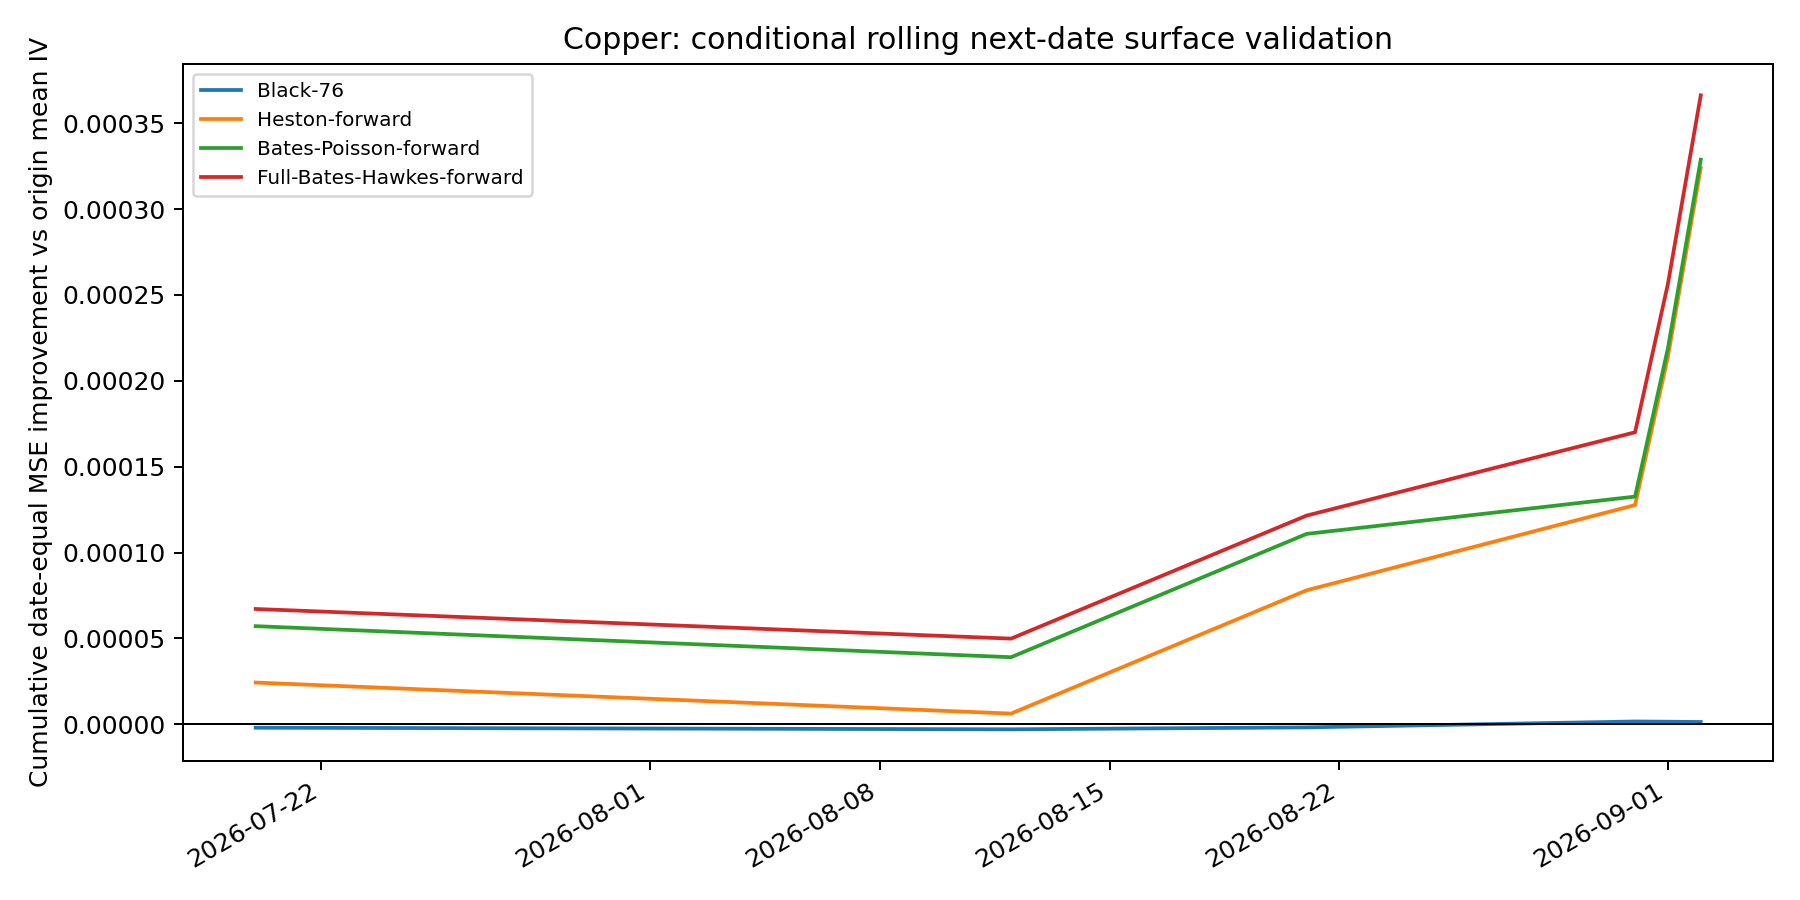
\includegraphics[width=.96\textwidth]{img/copper/copper_temporal_oos.png}
\caption{Cumulative date-equal MSE improvement against origin-mean IV. Only actual admitted targets enter; elapsed gaps are preserved. Positive improvement against this benchmark need not imply improvement against surface persistence.}
\label{fig:copper-temporal-oos}
\end{figure}
}{%
\gapbox{Historical copper acquisition and temporal validation are in progress.
The first static valuation is not temporally validated. Admit final coverage,
actual origin--target scores and the new paired valuation only from completed,
hash-verified local runs.}}

\chapter{A Three-Stage DCF Framework for Mining Valuation}
\chapterstatus{Expanded reconstruction from Team 5. The original article
provides accounting reclassification, FCFF/FCFE, WACC, three-stage transition
and a reproducible synthetic Monte Carlo illustration. This chapter retains
those supported methods, corrects the terminal-value cash-flow definition and
adapts the framework to a finite-resource miner. Synthetic values are never
reported as Barrick estimates.}

\section{Valuation object: firm value before equity value}

% Sources: Team 5 ch-2, ch-4 and 3df; CONTENT-LEDGER BG-U-11.
Discounted cash flow is not one formula but a consistency system linking a
cash-flow definition, the claim being valued and the corresponding discount
rate. Team 5 distinguishes two coherent routes. The equity route discounts
free cash flow to equity at the cost of equity,
\begin{equation}
EqV_0=\sum_{y=1}^{H}\frac{FCFE_y}{\prod_{s=1}^{y}(1+k_{e,s})}
      +\frac{TV_H^{Eq}}{\prod_{s=1}^{H}(1+k_{e,s})},
\end{equation}
whereas the firm route discounts FCFF at WACC and values all operating claims
before financing:
\begin{equation}
EV_0=\sum_{y=1}^{H}\frac{FCFF_y}{\prod_{s=1}^{y}(1+w_s)}
     +\frac{TV_H^{Firm}}{\prod_{s=1}^{H}(1+w_s)}.
\end{equation}
The unified experiment adopts the firm route because the Team 4 operating
layer produces pre-financing drivers. For scenario \(m\), enterprise value is
converted to equity and then to a per-share quantity only through an explicit
bridge:
\begin{align}
EqV^{(m)}
  &=EV^{(m)}-\text{net debt}-\text{minority and other claims}
    +\text{admitted non-operating assets},\\
V_{ps}^{(m)}&=\frac{EqV^{(m)}}{N_{dil}}.
\end{align}
The signs, scale, currency, security and date of every bridge item are part of
the valuation result. A direct FCFE calculation cannot be used to hide an
unreconciled capital structure.

For the attributable perimeter of Section~\ref{sec:company-financial-perimeter},
the generic bridge requires a basis check: mine-level partners' interests
already excluded from the operating flows must not be deducted again as
non-controlling interests. Consolidated cash, debt and other claims must be
mapped to those flows and corporate-level obligations. The zero placeholders
in the frozen numerical experiment do not perform that reconciliation.
Its diluted-share proxy allocates a subset operating value across whole-company
shares and cannot establish a corporate fair value. The copper extension
therefore reports aggregate values only.

The gold component margin multiplies production by a CoS measure defined per
ounce sold and containing depreciation, royalties and production taxes.
It is neither EBITDA nor fully reconciled EBIT. Separate sales/inventory,
D\&A, royalty response, working-capital and sustaining/growth-capital bridges
are required. Tanzania's legal ownership and economic-sharing agreement and
Loulo--Gounkoto's exceptional 2025Q4 cost anchor are additional checks;
their identification does not silently normalise the frozen inputs.

\begin{table}[H]
\centering
\small
\begin{tabularx}{\textwidth}{@{}p{2.7cm}p{3.0cm}p{2.8cm}X@{}}
\toprule
Route & Cash flow & Discount rate & Output and principal consistency test \\
\midrule
Firm valuation & FCFF before debt service & WACC & Enterprise value; operating
cash flows must exclude financing and be reconciled to invested capital. \\
Equity valuation & FCFE after net borrowing & Cost of equity & Equity value;
leverage policy and net borrowing must be modelled explicitly. \\
\bottomrule
\end{tabularx}
\caption{The two DCF routes recovered from Team 5. Mixing FCFF with the cost of
equity, or FCFE with WACC, changes the claim being valued and is inadmissible.}
\label{tab:dcf-route-consistency}
\end{table}

\section{Reclassifying financial statements for valuation}

% Sources: Team 5 ch-3; GAP-DCF-01 and GAP-VAL-05.
Standard statements mix operating, non-operating and financing items. Team 5's
reclassification is therefore a prerequisite, not an optional presentation
step. The operating side of invested capital can be expressed as
\begin{equation}
IC_y=OWC_y+PP\&E_y+\text{other net operating assets}_y,
\end{equation}
after excluding excess cash, marketable securities and other admitted
non-operating assets. The financing side must reconcile to debt and equity
claims. Return on invested capital is then
\begin{equation}
ROIC_y=\frac{NOPAT_y}{IC_{y-1}},
\end{equation}
so the comparison \(ROIC_y-w_y\) measures value creation from operating
capital rather than accounting earnings alone.

Operating working capital excludes cash and debt items that belong to the
financing bridge. In a mining application, inventories, receivables, payables,
royalties, reclamation provisions, streaming obligations and tax balances
must be assigned consistently. PP\&E and mine development also require care:
depreciation is an accounting allocation, sustaining capex is a cash outflow,
and closure liabilities are neither interchangeable nor automatically
contained in AISC.

NOPAT isolates after-tax operating profit from financing:
\begin{equation}
NOPAT_y=EBIT_y-\text{operating cash taxes}_y
       \approx EBIT_y(1-\tau_y),
\end{equation}
where the approximation is valid only when the tax rate and deferred-tax
adjustments are appropriate to the operating perimeter. Interest expense,
interest tax shields and income on excluded assets do not belong in NOPAT.

\begin{table}[H]
\centering
\small
\renewcommand{\arraystretch}{1.10}
\begin{tabularx}{\textwidth}{@{}p{3.0cm}p{4.2cm}X@{}}
\toprule
Block & Valuation treatment & Mining-specific control \\
\midrule
Revenue and operating cost & Build EBIT before financing. & Reconcile ounces,
realised price, ownership, royalties and whether cost metrics include D\&A or
sustaining investment. \\
Working capital & Include operating receivables, inventories and payables. &
Do not treat cash, debt or financing balances as operating working capital. \\
PP\&E and development & Link depreciation, capex and asset base. & Separate
sustaining, growth and closure expenditure; avoid counting AISC and capex
twice. \\
Taxes & Estimate operating cash taxes. & Separate current/deferred taxes,
jurisdictional effects and financing tax shields. \\
Non-operating and financing items & Exclude from FCFF and admit through the
EV-to-equity bridge. & Reconcile cash, debt, minorities, streams, other claims
and diluted shares to one filing date. \\
\bottomrule
\end{tabularx}
\caption{Financial-statement reclassification required before the operating
simulation can be called an FCFF model.}
\label{tab:dcf-reclassification}
\end{table}

\section{Operating forecasts and the FCFF contract}

% Sources: Team 5 ch-4 and ch-5; Team 4 interface.
Team 5 starts from sales, costs, margins, depreciation and working capital.
For a miner, the generic sales-growth shortcut is replaced by the more
informative component identity
\begin{equation}
Revenue_y^{(m)}=Q_y^{(m)}P_y^{realised,(m)}+\text{other operating revenue}_y^{(m)},
\end{equation}
where production \(Q\), realised price \(P^{realised}\), ownership and hedging
must share units and period conventions. Cost ratios can still be used as
checks, but a constant COGS-to-sales assumption is weak when grades, strip
ratios, energy, labour and mine mix change independently of price.

The admitted cash-flow identity is
\begin{align}
\text{Reinvestment}_y^{(m)}
  &=CapEx_y^{(m)}-D\&A_y^{(m)}+\Delta NWC_y^{(m)},\\
FCFF_y^{(m)}
  &=NOPAT_y^{(m)}-\text{Reinvestment}_y^{(m)}.
\end{align}
Every component uses the same sign convention: a rise in operating working
capital consumes cash, depreciation is non-cash, and capex consumes cash. CoS,
cash cost, AISC, royalties and D\&A cannot be combined until a data dictionary
proves what each aggregate already contains.

Team 5 also links growth to investment productivity. If expected operating
growth is \(g_y\) and the return on new invested capital is represented by
\(ROIC_y\), then
\begin{equation}
\text{reinvestment rate}_y=\frac{g_y}{ROIC_y},
\qquad
FCFF_y=NOPAT_y\left(1-\frac{g_y}{ROIC_y}\right).
\end{equation}
This identity prevents a model from assuming growth without funding it. It is
a consistency check rather than a licence to estimate Barrick's growth or
ROIC from the gold or equity-price series.

\section{Discount rate: currency, risk and capital structure}

% Sources: Team 5 ch-6; GAP-VAL-03/08.
Under the firm route, the pathwise or dated WACC is
\begin{equation}
w_y=\frac{E_y}{D_y+E_y}k_{e,y}
  +\frac{D_y}{D_y+E_y}k_{d,y}(1-\tau_y).
\end{equation}
A conventional CAPM estimate writes
\begin{equation}
k_{e,y}=R_{f,y}+\beta_y ERP_y+CRP_y,
\end{equation}
where any country-risk premium must match the geographic exposure and must not
be counted again in cash-flow haircuts. Beta requires an explicit convention:
a raw historical regression, smoothed beta or bottom-up unlevered/relevered
peer beta can produce different answers. The cost of debt may come from a
traded yield, recent borrowing spread or synthetic rating, but it must reflect
the same currency and horizon as the cash flows.

The risk-free input is conceptually a default-free zero-coupon rate matched to
the cash-flow maturity. A single long bond is only a proxy. Capital weights
should use market values and a target structure coherent with the forecast,
not book weights selected for convenience. If option-implied risk is already
embedded in the scenario distribution, the measure policy must also explain
why discounting does not charge for the same risk twice.

\section{Three stages and gradual convergence}

% Sources: Team 5 3df and montecarlo_int.
The three-stage model separates a high-growth or explicit phase, a transition
phase and a stable or closing phase. Its central contribution is gradual joint
convergence. Growth, operating margin, reinvestment, ROIC, leverage and risk
cannot jump independently at the terminal date. For a driver \(x\) that moves
from \(x_{hg}\) at the end of the first phase to \(x_s\) at year \(H\), a
transparent linear transition is
\begin{equation}
x_y=x_{hg}-\frac{y-H_1}{H-H_1}(x_{hg}-x_s),
\qquad H_1<y\leq H.
\end{equation}
The same device may be applied to several drivers, but their joint path must
remain economically coherent: lower growth normally implies lower incremental
reinvestment; mature margins and ROIC must be supportable; beta, leverage and
WACC should converge toward a defensible long-run state.

When perpetual continuation is economically admissible, Team 5's terminal
block is corrected to use post-horizon free cash flow rather than EBIT alone:
\begin{equation}
TV_H^{(m)}=
\frac{NOPAT_{H+1}^{(m)}
\left(1-g_s^{(m)}/ROIC_s^{(m)}\right)}
{w_H^{(m)}-g_s^{(m)}},
\qquad w_H^{(m)}>g_s^{(m)}.
\end{equation}
The denominator condition is necessary but not sufficient. Stable growth must
remain compatible with the valuation currency, long-run economy, reinvestment
capacity and return on new capital.

\section{Executable assumption register for the current experiment}
\label{sec:executable-valuation-assumptions}

The equations above describe the reusable method; this section discloses the
numbers actually passed to the current unified run. They are read from
the common September valuation input contract, not inferred
from the plotted valuation output. All four price branches use the same values.
They are deliberately classified as methodological assumptions because no
filing-level WACC, invested-capital reconstruction or mine-closure calibration
currently supports them as Barrick point estimates.

\begin{table}[H]
\centering
\caption{Editable non-gold parameters used by the current executable valuation.}
\label{tab:current-editable-valuation-parameters}
\scriptsize
\setlength{\tabcolsep}{3pt}
\renewcommand{\arraystretch}{1.10}
\begin{tabularx}{\textwidth}{@{}p{3.15cm}p{1.35cm}X X@{}}
\toprule
Configuration field & Current & Where it enters & Interpretation and effect \\
\midrule
\texttt{model.tax\_rate} & 25.0\% & Converts component margin to an
after-tax proxy. & Higher tax lowers explicit and terminal FCFF. \\
\texttt{model.high\_growth} & 8.5\% & First point of the five-year linear
growth schedule. & Raises early reinvestment through \(g/ROIC\); it does not
directly grow the operating margin paths. \\
\texttt{model.stable\_growth} & 2.5\% & Last schedule point and terminal
growth \(g_s\). & Changes terminal reinvestment and the \(w-g\) denominator. \\
\texttt{model.roic\_high} & 14.5\% & First point of the ROIC schedule. & At
fixed growth, higher ROIC reduces required reinvestment. \\
\texttt{model.roic\_stable} & 10.5\% & Last ROIC and terminal return. & Sets
terminal reinvestment \(g_s/ROIC_s=23.81\%\). \\
\texttt{model.wacc\_0} & 9.1\% & Initial state of the WACC process. & Affects
the conditional path from which years 1--5 are drawn. \\
\texttt{model.wacc\_long\_run} & 8.3\% & Mean-reversion level. & Pulls later
discount rates toward 8.3\%. \\
\texttt{model.wacc\_reversion} & 0.45 & Annual reversion speed. & Controls how
quickly the initial 9.1\% approaches the long-run level. \\
\texttt{model.wacc\_volatility} & 0.9\% & Diffusion scale of annual WACC. &
Widens the discount-rate and terminal-value distributions. \\
\texttt{model.terminal\_}\newline\texttt{spread\_floor} & 1.0\% & Lower-bound distance above
stable growth. & Enforces \(w_y\geq g_s+1\%=3.5\%\), with a separate 25\% cap. \\
\texttt{equity\_bridge.*} & zeros & EV-to-equity bridge. & Debt, cash,
minorities, other claims and non-operating assets are unresolved placeholders. \\
\texttt{diluted\_shares\_mn} & 1,675.51 & Equity value per share. & Unreconciled
proxy; changing it rescales every per-share distribution. \\
\bottomrule
\end{tabularx}
\end{table}

The five annual schedule points are generated by \texttt{numpy.linspace}.
Growth therefore moves through 8.5\%, 7.0\%, 5.5\%, 4.0\% and 2.5\%; ROIC moves
through 14.5\%, 13.5\%, 12.5\%, 11.5\% and 10.5\%. The corresponding
reinvestment rates are 58.62\%, 51.85\%, 44.00\%, 34.78\% and 23.81\%.
Figure~\ref{fig:current-dcf-driver-schedule} is generated by the valuation code
from those exact run inputs, and its CSV/JSON sidecars retain every plotted
number and field name.

\IfFileExists{img/valuation/dcf_driver_schedule.png}{%
  \begin{figure}[H]
    \centering
    \includegraphics[width=0.98\textwidth]{img/valuation/dcf_driver_schedule.png}
    \caption{Growth, ROIC and implied reinvestment schedule used by the current
    run. These common DCF assumptions do not vary across the four gold-price
    engines.}
    \label{fig:current-dcf-driver-schedule}
  \end{figure}
}{%
  \gapbox{The generated DCF-driver dashboard is unavailable; no editorially
  reconstructed substitute is admitted.}%
}

The annual WACC is not a manually descending list. Starting from \(w_0=9.1\%\),
the code applies
\begin{align}
w_{y+1}&=\bar w+(w_y-\bar w)e^{-\kappa}
       +\sigma_c\varepsilon_{y+1},\\
\sigma_c&=\sigma_w
\sqrt{\frac{1-e^{-2\kappa}}{2\kappa}},
\end{align}
with \(\bar w=8.3\%\), \(\kappa=0.45\), \(\sigma_w=0.9\%\) and independent
standard-normal shocks. The zero-shock path is approximately 8.81\%, 8.63\%,
8.51\%, 8.43\% and 8.38\% for years 1--5. The actual valuation uses 8,192
stochastic WACC paths, created once with seed 20260902 and reused byte-for-byte
under every gold model. Thus the shaded interval in
Figure~\ref{fig:current-wacc-assumption-paths} is discount-rate uncertainty,
whereas differences between model valuation distributions still isolate the
price engine.

\IfFileExists{img/valuation/fig_wacc_assumptions.png}{%
  \begin{figure}[H]
    \centering
    \includegraphics[width=0.95\textwidth]{img/valuation/fig_wacc_assumptions.png}
    \caption{Initial WACC, zero-shock mean-reversion path, simulated
    P10--P90 envelope, 8.3\% long-run level and terminal-spread floor used in
    the common valuation layer.}
    \label{fig:current-wacc-assumption-paths}
  \end{figure}
}{%
  \gapbox{The generated WACC-assumption dashboard is unavailable; no
  substitute path is supplied manually.}%
}

The terminal block applies the final positive after-tax component margin,
grows it once, funds stable growth at \(g_s/ROIC_s\), capitalises the resulting
FCFF at \(w_H-g_s\), and then discounts it back over the same path. The left
panel of Figure~\ref{fig:current-terminal-value-mechanics} makes the two most
sensitive editable inputs visible without pretending that the normalized
multiple is a company estimate. The right panel uses the accepted run and
reports how much of positive enterprise value comes from the discounted
terminal block under each price engine. This is the appropriate place to judge
whether the five-year horizon leaves excessive weight in the terminal value.

\IfFileExists{img/valuation/fig_terminal_multiple.png}{%
  \begin{figure}[H]
    \centering
    \includegraphics[width=0.49\textwidth]{img/valuation/fig_terminal_multiple.png}\hfill
    \includegraphics[width=0.49\textwidth]{img/valuation/fig_terminal_share.png}
    \caption{Terminal-value mechanics. Left: normalized sensitivity to stable
    growth and terminal WACC at the current stable ROIC. Right: actual-run
    P10, median and P90 terminal contribution to positive enterprise-value
    paths in the September refresh. Median shares are 78.26\%, 78.31\%,
    78.43\% and 78.27\% for Black--Scholes, Heston, Bates and Full Bates--Hawkes.}
    \label{fig:current-terminal-value-mechanics}
  \end{figure}
}{%
  \gapbox{The generated terminal-value dashboard is unavailable; no manually
  reconstructed sensitivity is admitted.}%
}

This register also clarifies how the project is joined. Team~8 changes only the
gold path; the Barrick/Team~4 operating vector is common; the tax,
growth--ROIC reinvestment rule, WACC array and terminal policy are common; and
the unresolved equity bridge is applied last. Consequently, editing any field
in Table~\ref{tab:current-editable-valuation-parameters} changes all four
branches together. Editing a Team~8 parameter changes only its corresponding
gold-price branch. No Team~4 simulated gold price or demonstrator valuation is
used.

\section{Finite-resource closure for a mining company}

Perpetual growth is not the automatic base case for a miner because reserves,
mine lives and closure obligations are finite. The terminal policy must connect
the explicit asset horizon to depletion, replacement, exploration and future
portfolio renewal. The alternatives in Table~\ref{tab:terminal-closure-alternatives}
are mutually exclusive modelling choices rather than terms to be blended.

\begin{table}[H]
\centering
\caption{Terminal-closure alternatives that must be chosen, not blended.}
\label{tab:terminal-closure-alternatives}
\small
\renewcommand{\arraystretch}{1.12}
\begin{tabularx}{\textwidth}{@{}p{3.00cm}X X@{}}
\toprule
Closure & Required evidence & Main risk \\
\midrule
Finite asset run-off & Mine lives, production decline, closure liabilities and
post-closure cash flows. & Omitting unmodelled replacement or corporate costs. \\
Explicit portfolio renewal & Exploration, development and acquisition
reinvestment tied to additions and future production. & Treating speculative
replacement as certain or costless. \\
Corporate going concern & Sustainable post-horizon FCFF, growth, ROIC, WACC
and continuing asset policy. & Hiding finite-resource economics inside a
perpetual-growth denominator. \\
\bottomrule
\end{tabularx}
\end{table}

\section{From deterministic DCF to a stochastic valuation distribution}

% Sources: Team 5 montecarlo_int, simulation_results and scenarios.
Team 5 extends the three-stage model without changing its accounting logic.
For each draw \(m\), it generates joint paths for operating drivers and WACC,
constructs FCFF, applies pathwise discount factors
\begin{equation}
DF_y^{(m)}=\prod_{s=1}^{y}\frac{1}{1+w_s^{(m)}},
\end{equation}
and returns
\begin{equation}
EV^{(m)}=\sum_{y=1}^{H}FCFF_y^{(m)}DF_y^{(m)}
       +TV_H^{(m)}DF_H^{(m)}.
\end{equation}
The reporting object is the empirical distribution
\(\{EV^{(1)},\ldots,EV^{(M)}\}\), summarised by its median, tail quantiles,
dispersion, terminal-value share and sensitivity measures. Dependence is part
of the model: weak operating states may coincide with higher discount rates,
and growth, margins, ROIC and reinvestment must move as a coherent narrative.

The accepted Team~5 contribution is methodological: distributions, fan
charts, terminal-value shares and driver attribution must be reported, and
Monte Carlo sampling error must be separated from economic dispersion. Its
standalone numerical example uses synthetic value units and is therefore
retained only as a branch-level implementation test. It is intentionally not
shown as Barrick evidence and contributes no simulated company price to the
unified valuation.

The scenario extension similarly varies coherent assumption sets rather than
one cell at a time. In the source illustration, conservative, base and
expansion cases jointly change growth, margin, ROIC, WACC and volatility. The
numerical values remain synthetic, but three methodological controls carry
into the thesis: every scenario must state its joint economic narrative; a
wider absolute distribution can accompany a stronger scenario; and the
terminal-value share must be reported because it can rise as stable economics
improve.

\section{Barrick-specific implementation contract}

The original Team 5 engine is a reproducible synthetic benchmark. It becomes
a Barrick valuation only after every illustrative driver is replaced by a
dated, unit-checked input and the finite-resource closure is selected. The
following table separates completed methodological reuse from open economic
reconciliation.

\begin{table}[H]
\centering
\caption{Team 5 contribution and Barrick-specific admission gate.}
\label{tab:dcf-reuse-gates}
\small
\renewcommand{\arraystretch}{1.12}
\begin{tabularx}{\textwidth}{@{}p{2.7cm}X X@{}}
\toprule
Element & Reusable contribution & Required before a validated Barrick claim \\
\midrule
Accounting perimeter & Operating/non-operating/financing reclassification,
NOPAT and invested-capital logic. & Filing-level mapping for Barrick, with
mining cost, D\&A, capex, tax and closure definitions reconciled. \\
FCFF engine & NOPAT, reinvestment and pathwise discounting identities. & Team
4-to-EBIT bridge, working capital, sustaining/growth capex and dimensional
tests. \\
WACC & Cost-of-equity/debt and capital-weight architecture. & Dated currency-
consistent risk-free curve, ERP, beta, borrowing spread, tax and market-value
weights. \\
Three-stage closure & Joint transition and growth--ROIC--reinvestment
consistency. & Mine horizon and one explicit, tested run-off, renewal or going-
concern policy. \\
Stochastic DCF & Distributional estimator, fan charts, quantiles, terminal
share and sensitivity reporting. & Approved joint scenarios, measure policy,
seeds, convergence and dependence diagnostics. \\
Equity bridge & Enterprise-versus-equity distinction. & Dated net debt, cash,
minorities, streams, other claims, non-operating assets and diluted shares. \\
\bottomrule
\end{tabularx}
\end{table}

The next chapter uses this architecture as a common contract across four gold-
price engines. It reports the conditional Barrick experiment and its validation
in one place; the calibration and predictive evidence itself remains in
Chapter~9 and is not repeated.

\chapter{Unified Barrick Valuation Experiment and Validation}
\chapterstatus{Unified version of the former valuation and validation
chapters. It reports one controlled comparison of four gold-price engines
under a common operating and DCF contract, then evaluates engineering,
numerical, accounting and external validity. Chapter~9 remains the sole home
of option calibration, residual geometry and out-of-sample forecasting, so
those results are referenced rather than repeated here.}

\section{End-to-end experiment contract}

The numerical experiment in this chapter is the frozen gold baseline:
company-wide actuals for 2026Q1--Q2 followed by the eight-mine forecast,
with the scope break disclosed in Chapter~10.
Section~\ref{sec:copper-extension} reports a separate extension
with three attributable copper operations, its own temporal validation
and a paired finite-horizon comparison. Gold-only per-share examples below
are not updated by adding a copper increment to their quantiles. The
extension first aggregates gold and copper on each path and reports
aggregate operating-value proxies without a reconciled equity bridge.

Chapter~11 defined the accounting, discounting and closure rules that must hold
before operating scenarios can become enterprise value, equity value and a
per-share quantity. The integrated experiment is therefore a sequence of typed
transformations rather than one black box:
\begin{align}
\mathcal P_{opt}^{\mathbb Q}
&\longrightarrow
\{S_{t,j}^{GLD,(m)},v_{t,j}^{(m)},N_{t,j}^{J,(m)},
\lambda_{t,j}^{H,(m)}\},\\
&\xrightarrow{\;\mathcal A_{scenario}\;}
\{P_{t,j}^{Au,(m)}\},\\
&\xrightarrow{\;\mathcal A_{operations}\;}
\{Rev_{y,j}^{(m)},\text{component margin}_{y,j}^{(m)}\},\\
&\xrightarrow{\;\mathcal A_{accounting}\;}
\{NOPAT_{y,j}^{(m)},FCFF_{y,j}^{proxy,(m)}\},\\
&\xrightarrow{\;\mathcal A_{DCF}\;}
\{EV_j^{(m)},EqV_j^{(m)},V_{ps,j}^{(m)}\},
\qquad j\in\{BS,H,BP,BH\}.
\end{align}
Each arrow has its own date, unit, measure and validation rule. Team 8 governs
the option-implied gold-price engines already developed and tested in
Chapter~9; Team~4 supplies the operating methodology and forecasts, refreshed
with Barrick actuals for 2026Q1--Q2; the unified DCF governs cash-flow
construction, discounting and the equity bridge; Team~3 supplies simulation
diagnostics. No source article alone authorises the last arrow.

\begin{table}[H]
\centering
\caption{Interfaces and stop conditions in the unified experiment.}
\label{tab:unified-interface-contract}
\scriptsize
\setlength{\tabcolsep}{3pt}
\renewcommand{\arraystretch}{1.10}
\begin{tabularx}{\textwidth}{@{}p{2.15cm}p{2.15cm}X X@{}}
\toprule
Stage & Source authority & Required contract & Stop condition \\
\midrule
Option scenarios & Teams 8 and 6 & Versioned snapshot, rate dates, parameter
objects, \(\mathbb Q\), time grid and seed. & A calibration or predictive
claim is inconsistent with Chapter~9. \\
Gold bridge & Team 8; unified adapter & Conditional transfer of
GLD/\(\mathbb Q\) distributional shape to gold USD/oz from one starting
level. & A GLD-level conversion, physical forecast or \(\mathbb Q\)-to-
\(\mathbb P\) transformation is implied rather than declared. \\
Operations & Team 4 & Production and cost units, ownership, frequency,
dependence and accounting definition. & CoS/AISC/D\&A/capex treatment or input
perimeter is ambiguous. \\
FCFF and closure & Team 5 & Taxes, reinvestment, WACC, horizon and terminal
policy. & Accounting identities, \(w>g\) or finite-resource closure fail. \\
Equity and per share & Team 5 plus corporate inputs & Net debt, minorities,
other claims, non-operating assets, diluted shares and matching listing. &
Bridge items do not reconcile to one dated filing and security. \\
Reporting & Teams 3 and 5; unified pipeline & Replay, quantiles, sensitivity
and hash-linked CSV/JSON/figure bundle. & A table and figure do not derive from
the same accepted run. \\
\bottomrule
\end{tabularx}
\end{table}

\section{Controlled design: one changing layer}

The experiment isolates the price-engine effect. It evaluates the four Team 8
engines named in Chapter~9 while holding production, unit costs, taxes, WACC,
terminal policy and equity inputs constant. Their stochastic laws and fit
diagnostics are not restated here. The relevant experimental fact is simpler:
only the gold-price scenario generator changes across the four branches.

The 20-quarter operating contract uses Barrick actual production and Cost of
Sales in 2026Q1--Q2, followed by Team~4 forecasts from 2026Q3. The actual and
forecast segments are labelled separately rather than presented as one
homogeneous source. Tax, growth, ROIC, stochastic WACC, terminal-growth and
equity-bridge inputs are common, and the same WACC shock array is reused in all
branches. Consequently, differences among the four output distributions can
be attributed to the gold-price engine within this common contract. They
cannot be attributed to mine plans, extraction uncertainty or cost inflation,
because those layers do not vary.

The exact editable values, their annual paths and their terminal-value effect
are disclosed once in Section~\ref{sec:executable-valuation-assumptions}, with
generated CSV/JSON sidecars. They are not repeated here: this chapter uses the
dashboard as the common downstream contract and focuses only on what changes
when the Chapter~9 gold engine changes.

The earlier Team~4 NSS, IV, GBM and stochastic EBITDA chain was a standalone
demonstrator. It is not imported into this experiment. Team~4 contributes only
the operating decomposition and forecast continuation; Team~8 alone generates
the current price paths. The current U.S. Treasury NSS term structure is a separate,
newly fitted Team~8/unified input and is therefore retained.

\section{Measure, dates and simulation design}

Option calibration identifies a risk-neutral law useful for market-implied
scenario analysis. It does not identify physical drift or a causal forecast of
realised gold. The adapter is therefore labelled a \emph{conditional transfer
of GLD/\(\mathbb Q\) distributional shape to gold USD/oz}. Each engine
restarts at USD~4,417/oz, Barrick's Q2 2026 average realised price used only
as a common level anchor. The procedure neither
converts GLD share levels into physical gold nor estimates a
\(\mathbb Q\)-to-\(\mathbb P\) map.

\paragraph{The operating law is not a measure change.}
For both gold and copper, denote the operating scenario law by $\mathcal R$.
It combines transferred option-implied coefficients, imposed commodity mean
schedules and an independent assumed WACC law. It is neither an estimated
physical law $\mathbb P$ nor the original traded-instrument pricing law
$\mathbb Q$. No Radon--Nikodym density or physical market-price-of-risk
specification is estimated. For a fixed-delivery futures price, the
deterministic-rate option convention uses zero drift; copper's
cross-delivery curve slope instead imposes a scenario mean and must not be
identified with that future's time drift. WACC shocks are not short-rate shocks.

In the jump simulators the compensator is
$\lambda(\mathbb E[e^J]-1)$ under the simulated mark law, with the left-step
intensity in Hawkes. A genuine measure transformation may change variance
drift, jump intensity and mark distribution as well as price drift; none is
identified by replacing a drift coefficient alone. Ordinary physical DCF
needs expected cash flows and a compatible risk-adjusted discount contract.
Pricing under $\mathbb Q$ needs the corresponding numeraire/pricing kernel
and treatment of non-spanned corporate risks. Q-shaped paths plus assumed
WACC can mix incompatible risk adjustments; substituting a risk-free rate
alone would not reconcile this corporate claim. The executable experiment
therefore admits only the conditional law $\mathcal R$ and rejects physical
or corporate risk-neutral interpretations. Unit-mean and nonzero-jump
compensation checks validate its numerical implementation, not its economics.

The date vector remains visible: the anchor quarter ends 30 June 2026, the
Treasury curve, Barrick close and current Team~8 surface are dated 2 September. The current surface is used for recalibration. The
remaining asynchrony restricts
the output to a conditional model comparison.

The numerical design uses 8,192 paths, 260 fine steps and 13 fine steps per
quarter over 20 quarters. All price engines use base seed 20260902; WACC uses
seed 20260902 and is generated once. The model-specific stream construction is
documented in Chapter~9. At the corporate layer, the important control is that
the same accepted operating arrays and WACC paths enter all branches.

\section{Executable method and result bundle}

% Generated fragments are admitted only from the authoritative final pointer.
\IfFileExists{chapters/generated/current-valuation-method.tex}{%
  \input{chapters/generated/current-valuation-method}%
}{%
  \gapbox{The accepted multi-model method fragment is unavailable. No
  substitute method claim is supplied editorially.}%
}

For \(M\) admitted paths from model \(j\), the empirical per-share
distribution and quantiles are
\begin{equation}
\widehat F_j(x)=\frac{1}{M}\sum_{m=1}^{M}
\mathbf 1\!\left\{V_{ps,j}^{(m)}\leq x\right\},
\qquad
\widehat Q_{u,j}=\inf\{x:\widehat F_j(x)\geq u\}.
\end{equation}
The table and figure below derive from the same versioned result bundle.

\IfFileExists{chapters/generated/current-valuation-multimodel-quantiles.tex}{%
  \input{chapters/generated/current-valuation-multimodel-quantiles}%
}{%
  \gapbox{The four-model quantile table is unavailable. No values are supplied
  editorially.}%
}

\IfFileExists{img/valuation/multimodel_value_distribution_comparison.png}{%
  \begin{figure}[H]
    \centering
    \includegraphics[width=0.98\textwidth]{img/valuation/multimodel_value_distribution_comparison.png}
    \caption{Kernel-density comparison of conditional Barrick value per share
    under the four Chapter~9 gold-price engines. Production, unit cost, DCF,
    WACC and equity inputs are common; the vertical line is the USD 44.13
    completed \texttt{B} close on 2 September 2026.}
    \label{fig:multimodel-value-distribution-comparison}
  \end{figure}
}{%
  \gapbox{The accepted four-model density comparison is unavailable until it
  is copied from the authoritative result manifest.}%
}

The medians are USD~35.87 for Black--Scholes/GBM, USD~35.67 for Heston,
USD~35.84 for Bates--Poisson and USD~35.14 for Full Bates--Hawkes. The
USD~44.13 close lies between the 58.08th and 59.24th model percentiles;
40.76--41.92\% of simulated values exceed it. Every branch places the observed
close above its conditional median but inside a broad distribution, not
establishing market mispricing.

P10 spans USD~3.13--3.71 and P90 USD~101.43--104.72. At more extreme quantiles,
P01 spans USD~-1.05 to USD~-0.34 and P99 USD~199.56--218.36. Negative proxy
quantiles are not forecasts of a negative limited-liability share price:
they expose the unreconciled corporate mapping. Fixed operations and DCF
compress median differences while preserving tail sensitivity.

\section{Layered validation}

Validation is not one score. Source parity, implementation tests, current-data
integrity, calibration, prediction, simulation stability and corporate
reconciliation answer different questions. The option-specific calibration
and chronological evidence is evaluated in Chapter~9. This section tests the
new information created by integration.

\IfFileExists{chapters/generated/current-valuation-diagnostics.tex}{%
  \input{chapters/generated/current-valuation-diagnostics}%
}{%
  \gapbox{The accepted diagnostic fragment is unavailable. No output may be
  promoted without deterministic replay, identity tests and manifest checks.}%
}

\begin{table}[H]
\centering
\caption{Evidence hierarchy for the integrated valuation.}
\label{tab:validation-evidence-hierarchy}
\scriptsize
\setlength{\tabcolsep}{3pt}
\renewcommand{\arraystretch}{1.10}
\begin{tabularx}{\textwidth}{@{}p{2.20cm}X X X@{}}
\toprule
Layer & Accepted evidence & Still open & Allowed conclusion \\
\midrule
Source integrity & Frozen hashes and admitted parity outputs for the eight
team modules. & Historical runtimes, licences and excluded assets recorded in
their source audits. & The admitted files are stable inputs, not independently
re-estimated facts. \\
Implementation & Team 8 and LSE boundary tests; unified complete and focused
suites; legacy/refactor equality in one runtime. & Full independent formula
review and all historical-market replay. & The tested contracts are
implemented within their declared tolerance. \\
Experiment identity & Same separated operating contract, unified DCF inputs and WACC paths in
all branches; monotone quantiles and pathwise bridge identities. & Stochastic
production/cost propagation and filing reconciliation. & Differences among
branches isolate price-engine sensitivity under the common contract. \\
Accounting & FCFF, discounting and per-share identities are executable. &
Actual debt, cash, minorities, other claims, share count and finite-mine
closure. & Outputs are conditional proxies rather than validated fair values. \\
External validity & Dates, units and \(\mathbb Q\)-scenario semantics are
serialized. & GLD-to-gold basis, \(\mathbb Q\)-to-\(\mathbb P\) bridge and
synchronous inputs. & The experiment is reproducible but not a physical gold
forecast. \\
\bottomrule
\end{tabularx}
\end{table}

\section{Numerical and simulation robustness}

The numerical gate covers analytical-pricer limits upstream, path-
discretisation bias, path-count convergence, seed stability, finite outputs,
quarterly aggregation and pathwise accounting identities. Monte Carlo error
and economic dispersion are distinct: the first concerns whether the numerical
estimator has converged; the second is the spread induced by the assumed
stochastic and corporate inputs.

The current refresh regression tests verify the snapshot contract and path
adapter; the versioned output preserves common operating and WACC input hashes.
Historical full-suite and 47-image audit counts describe the August bundle,
not a fresh validation of every September figure. Quantile ordering and the
pathwise corporate identities are separate from economic model validity.

These gates make the four distributions comparable computational outputs.
They do not validate the economic adapters through which GLD option scenarios
become gold revenue and then Barrick equity.

\section{Accounting and economic validation}

The current experiment keeps one operating vector deterministic after the
explicit actual/forecast handoff. That design supports attribution but
suppresses production and cost uncertainty. The unified DCF is likewise a common research contract, not a
filing-reconciled model. Debt, cash, minority interests, non-operating assets
and other claims remain zero placeholders, while 1,675.51 million diluted
shares are not reconciled to a common filing date. Equality of enterprise and
equity value in the run is therefore an input consequence, not a conclusion
about Barrick's balance sheet.

Economic validation must additionally reconcile revenue to volumes and
realised prices; operating margin to EBIT; NOPAT, reinvestment and FCFF by path
and year; positive discount factors; admissible terminal denominators; and the
EV-to-equity adjustments described in Chapter~11. Sensitivities must use native
units and follow directions implied by the equations. No option-pricing fit can
substitute for these controls.

\section{External validity and information limits}

GLD option values, the GLD share price, physical gold in USD/oz, Barrick's
realised selling price and mine-level cash flow are distinct objects. The run
transfers the shape of a GLD/\(\mathbb Q\) distribution to paths restarted at
the USD~4,417/oz Barrick realised-price anchor without a validated
physical-measure map. The
asynchronous dates listed above remain a limitation after every software test
passes.

The information set also excludes timestamped macroeconomic and geopolitical
news. Such events may enter indirectly through prices, implied volatility and
jumps, but the current filtration cannot identify their causal contribution.
An NLP or machine-learning extension is therefore a genuine future research
question requiring leakage controls and chronological evaluation, not an
unfinished step of the present valuation.

\section{What the integrated experiment establishes}

The combined result is intentionally bounded. The project has completed the
planned integration of the Team~8 price layer, separated Team~4/Barrick
operating layer and unified stochastic DCF contract. Under one common set of operating and corporate
assumptions, all four price engines place the USD 44.13 close above their
conditional medians while retaining substantial probability mass above it.
The close remains inside every broad distribution, so the common direction is
a scenario result rather than evidence of mispricing.

The experiment also identifies where model form matters: price-engine choice
changes tail geometry more than the median under this common downstream
contract. What remains open is not the act of integration itself, but the
economic validation of its commodity, measure, operating, accounting and
terminal-closure interfaces. The unnumbered conclusion that follows separates
those limitations from the next genuinely new research programme.

\chapter*{Conclusion and Future Research}
\addcontentsline{toc}{chapter}{Conclusion and Future Research}
\markboth{Conclusion and Future Research}{Conclusion and Future Research}
\chapterstatus{Unnumbered synthesis of findings, present limitations and
genuinely new research directions. Items already completed by the unified
project are recorded as results rather than repeated as future work.}

\section*{What the project has completed}

This thesis converts eight specialised studies into one traceable research
architecture. Its main contribution is the separation and subsequent
connection of five objects: the historical gold series, the option-implied
gold-price law, production, unit cost and corporate cash flow. The resulting
chain is explicit enough to identify which evidence supports each output and
where a change of data, units, measure or accounting perimeter occurs.

Several tasks described as future work in the standalone articles are now
complete. The Team 8 project no longer stops at Black--Scholes, Heston or
independent Bates jumps: it contains the full affine Bates--Hawkes
specification, constrained calibration, residual and smile diagnostics,
four-model path simulation and a dense-only rolling comparison over 30 origins and 4,667 common forecasts. Its
price scenarios have also been connected to Barrick 2026Q1--Q2 actuals, the
Team~4 forecast from 2026Q3 and the unified DCF/WACC/equity contract. The
Team~4 price demonstrator is excluded. The valuation is therefore an implemented
four-branch experiment, not a proposed future integration.

Under that common contract, the four conditional Barrick medians lie between
USD~35.14 and USD~35.87 per share, below the completed USD~44.13 close
on 2 September 2026. The close remains inside every broad distribution,
with 40.76--41.92\% of simulated values above it. Full Bates--Hawkes is the
primary OOS-ranked structural scenario and gives a median of USD~35.14,
whereas Heston is the current-snapshot fit winner. The shared direction
is a property of the admitted assumptions, not evidence of market mispricing.

The comparison further shows that changing the gold-price law affects the
tails more than the central corporate value when production, cost, WACC and
the equity bridge are fixed. This is a useful attribution result: it identifies
where price-model complexity propagates through the DCF and where downstream
assumptions compress or dominate its effect.

\section*{Present limitations}

The completed integration remains conditional at several economic interfaces.
First, GLD option dynamics are estimated under \(\mathbb Q\), whereas a
long-horizon operating valuation would ideally use scenarios justified under
\(\mathbb P\). Restarting the option-implied engines at a physical-gold level
transfers distributional shape; it is not a validated GLD-to-gold conversion
or change of measure. The gold start, Treasury curve, calibration surface,
Barrick close and current surface audit are explicitly dated: the market snapshot is 2 September, while the realised-price anchor is a Q2 average.

Second, the unified run uses Barrick actuals only for 2026Q1--Q2 and fixes the
Team~4 forecast thereafter. That design isolates price-engine risk but does not propagate reserve,
grade, recovery, energy, labour, mine-mix or closure uncertainty. Dependence
between gold prices and operating conditions is therefore not estimated.

Third, Team 5 supplies a coherent DCF architecture rather than a
filing-reconciled Barrick model. The operating-to-EBIT bridge, cash taxes,
working capital, sustaining and growth capex, debt, cash, minorities, streams,
other claims, non-operating assets and diluted shares require one dated
corporate reconciliation. The present zero bridge items and share-count proxy
are assumptions. Finite-mine closure also remains less developed than the
generic going-concern terminal block.

Finally, a sophisticated stochastic law does not eliminate model risk. The
current cross-section favours Heston, whereas Full Bates--Hawkes leads the rolling OOS ranking. Its branching ratio is 0.5569, not the former August floor. No model beats interpolated IV persistence. Parameter pressure,
surface sampling, optimizer dependence, regime shifts and the choice of
physical-measure transformation remain sources of uncertainty.

Costs retain a persistent trend without additional technology-driven reductions.
This is prudential relative to otherwise identical efficiency-improvement
scenarios, not a mathematical lower bound. Stochastic operating costs would
introduce favourable and adverse outcomes, and their conditional mean could
remain smooth. Productivity improvements and their investment costs must be
evaluated jointly with the growth already included in the DCF.

\section*{Future research programme}

The next research cycle should begin with economic reconciliation rather than
another layer of stochastic complexity. A dated Barrick data contract should
map mine-level production, realised prices, royalties, cash costs, AISC,
depreciation, sustaining and growth capex, working capital, taxes and closure
liabilities into EBIT, invested capital and FCFF. Debt, cash, minority
interests, streams, non-operating assets and diluted shares should then close
the EV-to-equity bridge to the same filing and listing.

The commodity interface requires a separate empirical programme. The GLD-to-
physical-gold basis should be estimated and stress-tested, and risk-neutral
option scenarios should be converted into physical scenarios through an
explicitly validated risk-premium or filtering model. Only after that step can
the long-horizon paths be interpreted as more than option-implied conditional
shapes.

Operating uncertainty should then be reintroduced jointly. Team 4 production
and cost models can be sampled alongside price, but their dependence structure
must be estimated or scenario-defined. Mine depletion, expansion projects,
reserve conversion, inflation, energy and foreign-exchange shocks should feed
an explicit finite-resource closure. The comparison can then be repeated to
measure whether gold-model choice or operating/accounting uncertainty explains
more of the equity-value distribution.

A later information layer may augment the filtration with timestamped
macroeconomic and geopolitical data. News embeddings, NLP classifications or
machine-learning forecasts are admissible only with event-time alignment,
leakage controls, pre-declared benchmarks and true chronological evaluation.
The relevant question is not whether a flexible model improves in-sample fit,
but whether incremental information improves forecasts beyond price,
volatility and persistence benchmarks.

Further model research may examine time-varying risk premia, regime-dependent
parameters, model averaging and a rough-Hawkes option-pricing construction.
Those extensions should be judged through the same hierarchy used here:
mathematical admissibility, deterministic implementation tests, dated
out-of-sample evidence and economic propagation through a reconciled corporate
model.

\section*{Concluding synthesis}

The project demonstrates the value of interdisciplinarity in applied finance.
Probability, stochastic calculus, econometrics, numerical methods,
optimization, accounting and corporate valuation are not parallel subjects in
this setting; each constrains a different interface of the same experiment.
The strongest outcome is therefore not one point estimate or one preferred
model. It is a reproducible framework that keeps historical evidence,
option-implied information, operating assumptions and accounting claims
separate until the moment they are deliberately connected.

Within that framework, Full Bates--Hawkes offers the richest admitted
description of current option-implied variance and clustered jumps, while the
four-model valuation shows how little a better surface fit alone can establish
about a mining company's equity. The thesis closes with a conditional result,
an explicit inventory of unresolved economic bridges and a research programme
capable of testing them. The copper extension of
Section~\ref{sec:copper-extension} expands the operating perimeter and adds
dated conditional surface tests, while leaving the accounting, realised-price,
mine-life and equity bridges explicit. Its aggregate paired values do not
supersede the gold-only per-share examples with a corporate target.
The study does not issue a fair-value certification, target
price or investment recommendation.


\begin{references}
\bibitem{team1}
Stefano Falcione and Marco Fracca, \emph{Black--Scholes Foundations}, Barrick project source article, supplied workspace copy.

\bibitem{team2}
Filippo Triassi and Giorgio Zoccatelli, \emph{OLS and Dynamic Correlations}, Barrick project source article, supplied workspace copy.

\bibitem{team3}
Andrea Rostagno and Francesco Florio, \emph{Monte Carlo Risk}, Barrick project source article, supplied workspace copy.

\bibitem{team4}
Giacomo Scali and Jacopo Foralosso, \emph{Component-Driven EBITDA}, Barrick project source article, supplied workspace copy.

\bibitem{team5}
Federico Vesco, Lorenzo Pietra and Bader Moussaif, \emph{Three-Stage DCF}, Barrick project source article, supplied workspace copy.

\bibitem{team6}
Davide Sisto and Matteo Armando, \emph{Beyond Black--Scholes}, Barrick project source article, supplied workspace copy.

\bibitem{team7}
Davide D'Amico and Pietro Weisz, \emph{Gold Volatility Dynamics}, Barrick project source article, supplied workspace copy.

\bibitem{team8}
Salvatore Gabriele Messina and Alessandro Coco, \emph{Gold Options Stochastic Modeling}, Barrick project source article, supplied workspace copy.

\bibitem{lse-2026}
London Strategic Edge, \emph{Market-data and options datasets}, provider snapshot accessed 28 August 2026. Aggregate statistics and derived figures are reported under the project's non-redistribution boundary.

\bibitem{barrick-name-2025}
Barrick Mining Corporation, \emph{Barrick Announces Name Change to Barrick Mining Corporation and Election of Directors}, 6 May 2025, \href{https://www.barrick.com/English/news/news-details/2025/barrick-announces-name-change-to-barrick-mining-corporation-and-election-of-directors/default.aspx}{official corporate release}.

\bibitem{barrick-about-2026}
Barrick Mining Corporation, \emph{About Barrick}, corporate profile accessed 27 August 2026, \href{https://www.barrick.com/English/about/default.aspx}{official company profile}.

\bibitem{barrick-ar-2025}
Barrick Mining Corporation, \emph{Annual Report 2025}, MD\&A (prepared
4 February 2026), Production Costs, mine tables and Notes 2, 4 and 35,
\href{https://s25.q4cdn.com/322814910/files/doc_financial/annual_reports/2025/Barrick_Annual_Report_2025.pdf}{official annual report}.

\bibitem{barrick-mine-stats-2026}
Barrick Mining Corporation, \emph{Q1 and Q2 2026 Mine Statistics},
\href{https://s25.q4cdn.com/322814910/files/doc_financial/quarterly_results/2026/q1/Barrick_Q1_2026_Mine_Stats.pdf}{Q1 tables}
and \href{https://s25.q4cdn.com/322814910/files/doc_financial/quarterly_results/2026/q2/Barrick_Q2_2026_Mine_Stats.pdf}{Q2 tables}.

\bibitem{ib-historical-limitations}
Interactive Brokers, \emph{TWS API: Historical Data Limitations},
\href{https://interactivebrokers.github.io/tws-api/historical_limitations.html}{API historical-data documentation},
accessed 3 October 2026. Availability is supplemented by actual read-only
historical bid/ask retrievals, whose local manifests retain timestamps and hashes.

\bibitem{barrick-ipo-2026}
Barrick Mining Corporation, \emph{Barrick Advances IPO of North American Gold
Assets, Announces Executive Appointments}, 28 April 2026,
\href{https://www.barrick.com/English/news/news-details/2026/barrick-advances-IPO-of-north-american-gold-assets/default.aspx}{official release}.

\bibitem{barrick-q2-release-2026}
Barrick Mining Corporation, \emph{Barrick Reports Second Quarter 2026 Results},
10 August 2026, \href{https://www.barrick.com/English/news/news-details/2026/q2-2026-results/default.aspx}{official release}.

\bibitem{imf-war-inflation-2022}
International Monetary Fund, \emph{War Dims Global Economic Outlook as Inflation Accelerates}, 19 April 2022, \href{https://www.imf.org/en/Blogs/Articles/2022/04/19/blog-weo-war-dims-global-economic-outlook-as-inflation-accelerates}{IMF analysis}.

\bibitem{ecb-gold-risk-2025}
European Central Bank, \emph{Gold demand: the role of the official sector and geopolitics}, Financial Stability Review, May 2025, \href{https://www.ecb.europa.eu/press/financial-stability-publications/fsr/focus/2025/html/ecb.fsrbox202505_02~7f616fcd3f.en.html}{ECB analysis}.

\bibitem{fed-gold-reserves-2025}
Board of Governors of the Federal Reserve System, \emph{Exploring Central Bank Gold Purchases and the Dollar's Role in International Reserves}, International Finance Discussion Papers, \href{https://www.federalreserve.gov/econres/ifdp/exploring-central-bank-gold-purchases-and-the-dollars-role-in-international-reserves.htm}{Federal Reserve paper}.

\bibitem{wgc-gdt-q2-2026}
World Gold Council, \emph{Gold Demand Trends Q2 2026: Central Banks}, accessed 27 August 2026, \href{https://www.gold.org/goldhub/research/gold-demand-trends/gold-demand-trends-q2-2026/central-banks}{demand report}.

\bibitem{github-placeholder}
Barrick Gold Research Teams, \emph{Stochastic Valuation of Barrick Mining: unified thesis and supporting code}, Starting Finance Club PoliTo, \href{https://github.com/StartingFinanceClubPoliTo/Research/tree/main/Barrick-Gold/Barrick\%20Mining\%20UNIFICATO}{Barrick Mining UNIFICATO repository}, accessed 29 August 2026.
\end{references}

\end{document}
